\documentclass[a4paper,11pt, twoside]{memoir}

\usepackage{lualatex-math}
\usepackage{amsmath}
\usepackage{unicode-math}
\usepackage{polyglossia}
\setdefaultlanguage[]{polish}
\defaultfontfeatures{Ligatures=TeX}

\usepackage[top=25mm, bottom=25mm, left=30mm, right=20mm]{geometry}
\usepackage[linktoc=section]{hyperref}
\hypersetup{verbose, pdfborder={0 0 0.2},   bookmarksopen=true ,bookmarksnumbered=true, colorlinks=false,  unicode=true}
\usepackage{bookmark}
\usepackage[usenames,dvipsnames]{color}
\usepackage{url}
\usepackage{listings}
\usepackage[sort, compress]{cite}
\usepackage{graphicx}
\usepackage[labelsep=period]{caption}
\usepackage{diagbox}
\usepackage{xfrac}
\usepackage{tabularx}
\usepackage{setspace}
\usepackage{fontspec}
\usepackage{siunitx, booktabs}
\usepackage{nicefrac}
\defaultfontfeatures{Ligatures=TeX}






%%%%%%%%%%%%%%%%%%%%%%%%%%%%%%%%%%%%%%%%%%%%%%%%%%%%%%%%%%%%%%%%%%%%%%%%%%%%%%%%%%%%%%%%%
%%% Wybór fontu)                                                                      %%%
%%%\setmainfont{TeX Gyre Pagella})                                                    %%%
\setmainfont{FreeSerif}                                                               %%%
%%%%%%%%%%%%%%%%%%%%%%%%%%%%%%%%%%%%%%%%%%%%%%%%%%%%%%%%%%%%%%%%%%%%%%%%%%%%%%%%%%%%%%%%%


%%%%%%%%%%%%%%%%%%%%%%%%%%%%%%%%%%%%%%%%%%%%%%%%%%%%%%%%%%%%%%%%%%%%%%%%%%%%%%%%%%%%%%%%%
%%% Definicje symboli i skrótów (początek)                                            %%%
\usepackage[toc, nonumberlist]{glossaries}                                            %%%
\usepackage{glossaries-extra}                                                         %%%
\setglossarystyle{listdotted}                                                         %%%
\setlength{\glslistdottedwidth}{25mm}                                                 %%%

\makenoidxglossaries                                                                  %%%
\loadglsentries{glossary.tex}                                                         %%%
\glsaddall                                                                            %%%
%%% Definicje symboli i skrótów (koniec)                                              %%%
%%%%%%%%%%%%%%%%%%%%%%%%%%%%%%%%%%%%%%%%%%%%%%%%%%%%%%%%%%%%%%%%%%%%%%%%%%%%%%%%%%%%%%%%%


%%%%%%%%%%%%%%%%%%%%%%%%%%%%%%%%%%%%%%%%%%%%%%%%%%%%%%%%%%%%%%%%%%%%%%%%%%%%%%%%%%%%%%%%%
%%% Pomocnicze makro definiujące elegancką werję  BibTeX                              %%%
\def\BibTeX{{\textrm B\kern-.05em{\textsc i\kern-.025em b}\kern-.08emT\kern-.1667em\lower.5ex\hbox{E}\kern-.125emX }}                         %%%
%%%%%%%%%%%%%%%%%%%%%%%%%%%%%%%%%%%%%%%%%%%%%%%%%%%%%%%%%%%%%%%%%%%%%%%%%%%%%%%%%%%%%%%%%


%%%%%%%%%%%%%%%%%%%%%%%%%%%%%%%%%%%%%%%%%%%%%%%%%%%%%%%%%%%%%%%%%%%%%%%%%%%%%%%%%%%%%%%%%
%%%   Tabele i rysunki                                                                %%%
%%%Parametr "rozciągający" komórki tabeli                                             %%%
%\renewcommand{\arraystretch}{1.2}                                                    %%%
                                                                                      %%%
%%% dodatkowy odstęp w tablicy                                                        %%%
\setlength\extrarowheight{2pt}                                                        %%%
                                                                                      %%%
%%% Format podpisów rysunków                                                          %%%
\captionsetup[figure]{skip=0pt, name=Rys.}                                            %%%
%%%%%%%%%%%%%%%%%%%%%%%%%%%%%%%%%%%%%%%%%%%%%%%%%%%%%%%%%%%%%%%%%%%%%%%%%%%%%%%%%%%%%%%%%


%%%%%%%%%%%%%%%%%%%%%%%%%%%%%%%%%%%%%%%%%%%%%%%%%%%%%%%%%%%%%%%%%%%%%%%%%%%%%%%%%%%%%%%%%
%%% Konfiguracja głębokości numeracji podrozdziałów
\setsecnumdepth{subsection}
\maxsecnumdepth{subsection}

%%% Konfiguracja głębokości spisu treści
%%% Dwa poziomy
\maxtocdepth{section}
%%% lub
%%% trzy poziomy 
%\maxtocdepth{subsection}

%%%Lokalizacja plików graficznych
%%%%%%%%%%%%%%%%%%%%%%%%%%%%%%%%%%%%%%%%%%%%%%%%%%%%%%%%%%%%%%%%%%%%%%%%%%%%%%%%%%%%%%%%%
\graphicspath{ {../grafika/} }
%%%%%%%%%%%%%%%%%%%%%%%%%%%%%%%%%%%%%%%%%%%%%%%%%%%%%%%%%%%%%%%%%%%%%%%%%%%%%%%%%%%%%%%%%


%%%%%%%%%%%%%%%%%%%%%%%%%%%%%%%%%%%%%%%%%%%%%%%%%%%%%%%%%%%%%%%%%%%%%%%%%%%%%%%%%%%%%%%%%

%%%%%%%%%%%%%%%%%%%%%%%%%%%%%%%%%%%%%%%%%%%%%%%%%%%%%%%%%%%%%%%%%%%%%%%%%%%%%%%%%%%%%%%%%

%%%%%%%%%%%%%%%%%%%%%%%%%%%%%%%%%%%%%%%%%%%%%%%%%%%%%%%%%%%%%%%%%%%%%%%%%%%%%%%%%%%%%%%%%
%%%  Parametry wpływające na skład tekstu                                             %%%
\clubpenalty=10000                                                                    %%%
\widowpenalty=10000                                                                   %%%
\brokenpenalty=10000                                                                  %%%
\sloppy                                                                               %%%
                                                                                      %%%
\tolerance4500                                                                        %%%
\pretolerance250                                                                      %%%
\hfuzz=1.5pt                                                                          %%%
\hbadness1450                                                                         %%%
%%%%%%%%%%%%%%%%%%%%%%%%%%%%%%%%%%%%%%%%%%%%%%%%%%%%%%%%%%%%%%%%%%%%%%%%%%%%%%%%%%%%%%%%%


%%%%%%%%%%%%%%%%%%%%%%%%%%%%%%%%%%%%%%%%%%%%%%%%%%%%%%%%%%%%%%%%%%%%%%%%%%%%%%%%%%%%%%%%%
%%% Definiowanie stylu strony (początek)                                              %%%
\chapterstyle{section}                                                                %%%
\copypagestyle{chapter}{ruled}                                                        %%%
\pagestyle{empty}                                                                     %%%
\makeevenhead{ruled}{}{}{}                                                            %%%
\makeoddhead{ruled}{}{}{}                                                             %%%
\makeheadrule{ruled}{0pt}{0pt}                                                        %%%
\setlength{\parindent}{5mm}                                                           %%%
%%%%%%%%%%%%%%%%%%%%%%%%%%%%%%%%%%%%%%%%%%%%%%%%%%%%%%%%%%%%%%%%%%%%%%%%%%%%%%%%%%%%%%%%%


%%%%%%%%%%%%%%%%%%%%%%%%%%%%%%%%%%%%%%%%%%%%%%%%%%%%%%%%%%%%%%%%%%%%%%%%%%%%%%%%%%%%%%%%%
%%% Symbole używane w listach                                                         %%%
\renewcommand{\labelitemi}{$\bullet$}                                                 %%%
\renewcommand{\labelitemii}{--}                                                       %%%
\renewcommand{\labelitemiii}{$\circ$}                                                 %%%
%%%%%%%%%%%%%%%%%%%%%%%%%%%%%%%%%%%%%%%%%%%%%%%%%%%%%%%%%%%%%%%%%%%%%%%%%%%%%%%%%%%%%%%%%


%%%%%%%%%%%%%%%%%%%%%%%%%%%%%%%%%%%%%%%%%%%%%%%%%%%%%%%%%%%%%%%%%%%%%%%%%%%%%%%%%%%%%%%%%
\definecolor{ListingBackground}{rgb}{0.95,0.95,0.95}                                  %%%
\lstset{ %language=VHDL,                                                              %%%
	basicstyle=\scriptsize,                                                           %%%
	frameround=ffff,                                                                  %%%
	keywordstyle={\bfseries\scriptsize},                                              %%%
	commentstyle={\em\scriptsize\color{Gray}},                                        %%%
	numbers=left,                                                                     %%%
	stepnumber=5,                                                                     %%%
	firstnumber=1,                                                                    %%%
	numberfirstline=true,                                                             %%%
	numberblanklines=true,                                                            %%%
	numberstyle={\tiny},                                                              %%%
	numbersep=10pt,                                                                   %%%
	tabsize=2,                                                                        %%%
	xleftmargin=20pt,                                                                 %%%
	framexleftmargin=3pt,                                                             %%%
	framexbottommargin=2pt,                                                           %%%
	framextopmargin=2pt,                                                              %%%
	framexrightmargin=0pt,                                                            %%%
	showstringspaces=true,                                                            %%%
	backgroundcolor={\color{ListingBackground}},                                      %%%
	extendedchars=true,                                                               %%%
	% title=\lstname,                                                                 %%%
	captionpos=t,                                                                     %%%
	% abovecaptionskip=1pt,                                                           %%%
	% belowcaptionskip=1pt,                                                           %%%
	frame=tb,                                                                         %%%
	framerule=0.2pt}                                                                  %%%
%%%%%%%%%%%%%%%%%%%%%%%%%%%%%%%%%%%%%%%%%%%%%%%%%%%%%%%%%%%%%%%%%%%%%%%%%%%%%%%%%%%%%%%%%


%%%%%%%%%%%%%%%%%%%%%%%%%%%%%%%%%%%%%%%%%%%%%%%%%%%%%%%%%%%%%%%%%%%%%%%%%%%%%%%%%%%%%%%%%
%%% Spolszczone/zmienione nazwy sekcji dokumentu                                      %%%
\renewcommand*\lstlistingname{Wydruk}                                                 %%%
\renewcommand*\lstlistlistingname{Spis wydruków}                                      %%%
                                                                                      %%%
\renewcommand{\appendixname}{Załącznik}                                               %%%
\renewcommand{\appendixpagename}{Załączniki}                                          %%%
%\renewcommand{\appendixpagename}{załączniki}                                          %%%

\renewcommand{\appendixtocname}{Spis załączników}
%%%%%%%%%%%%%%%%%%%%%%%%%%%%%%%%%%%%%%%%%%%%%%%%%%%%%%%%%%%%%%%%%%%%%%%%%%%%%%%%%%%%%%%%%


\renewcommand\mempostaddapppagetotochook{\cftinserthook{toc}{BREAK}}
\cftinsertcode{BREAK}{\changetocdepth{-10}}
\let\normalchangetocdepth\changetocdepth
% needed for late

\makeatletter
\newcommand\appendixtableofcontents{
\begingroup
\let\changetocdepth\@gobble
\normalchangetocdepth{-10}
\cftinsertcode{BREAK}{\normalchangetocdepth{3}}
\renewcommand\contentsname{Spis załączników}
\tableofcontents*
\endgroup
}
\makeatother

%\newcommand{\listanswername}{Spis załączników}
%\newlistof{listofanswers}{zalaczniki}{\listanswername}
%
%\newcounter{answer}[chapter]
%\renewcommand{\theanswer}{\arabic{answer}}
%\newcommand{\answer}[1]{
%\refstepcounter{answer}
%\par\noindent\textbf{Answer \theanswer. #1}
%\addcontentsline{ans}{answer}{\protect\numberline{\theanswer}#1}\par}



\begin{document}
%%%%%%%%%%%%%%%%%%%%%%%%%%%%%%%%%%%%%%%%%%%%%%%%%%%%%%%%%%%%%%%%%%%%%%%%%%%%%%%%%%%%%%%%%
%%%%%%%%%%%%%%%% Parametry strony tytułowej  %%%%%%%%%%%%%%%%%%%%%%%%%%%%%%%%%%%%%%%%%%%%
%%%%%%%%%%%%%%%%%%%%%%%%%%%%%%%%%%%%%%%%%%%%%%%%%%%%%%%%%%%%%%%%%%%%%%%%%%%%%%%%%%%%%%%%%
\newcommand\rok{2017}
\newcommand\rodzajpracy{Praca dyplomowa \\ \vskip6pt inżynierska}
%\newcommand\rodzajpracy{Praca dyplomowa \\ \vskip6pt magisterska}
\newcommand\kierunek{Elektronika, Informatyka i Telekomunikacja}
\newcommand\specjalnosc{Elektronika i inżynieria komputerowa}
\newcommand\tytulpl{Optymalizacja nieoptymalnych rozwiązań w~celu uzyskania dyplomu}
\newcommand\tytulen{Optimization of non-optimal solutions in order to get a~diploma}
\newcommand\autor{Adam Kowalski}
\newcommand\nralbumu{123456789}
\newcommand\promotor{prof. dr hab. Iks Igrekowski}
%%%%%%%%%%%%%%%%%%%%%%%%%%%%%%%%%%%%%%%%%%%%%%%%%%%%%%%%%%%%%%%%%%%%%%%%%%%%%%%%%%%%%%%%%


%%%%%%%%%%%%%%%%%%%%%%%%%%%%%%%%%%%%%%%%%%%%%%%%%%%%%%%%%%%%%%%%%%%%%%%%%%%%%%%%%%%%%%%%%
%%%%%%%%%%%%%%%%%%%%%%%%%%%%%%%%%%%%%%%%%%%%%%%%%%%%%%%%%%%%%%%%%%%%%%%%%%%%%%%%%%%%%%%%%
%%% wczytanie pliku z formatem strony tytułowej
\thispagestyle{empty}

{ \centering

{ %\setmainfont{t1xtt} 
%\setmainfont[]{Belgrano Regular} %\ttfamily 
\setmainfont{Latin Modern Mono}
%\setmainfont{Noto Serif}
\begin{minipage}[c]{\textwidth}
\centering
\begin{minipage}[c]{0.65\textwidth}   \centering
{\fontsize{23pt}{36pt}\selectfont {Politechnika Warszawska}} \vskip 4pt 
{\setmainfont[LetterSpace=35]{Latin Modern Mono} \fontsize{12pt}{24pt}   \selectfont  
 {WYDZIAŁ \hskip12pt ELEKTRONIKI \\  I \hskip12pt TECHNIK \hskip12pt INFORMACYJNYCH}}
\end{minipage}
\begin{minipage}[c]{0.18\textwidth}
\centering

\includegraphics[height=25mm]{pwlogo.png}
\end{minipage}
\end{minipage}
}

\vfill

{\setmainfont{Noto Sans} 
\begin{minipage}[c]{\textwidth}   \centering
{\fontsize{12pt}{24pt}\selectfont Instytut Mikroelektroniki i Optoelektroniki}
\end{minipage}}

\vfill

{ %\setmainfont{t1xtt} 
%\setmainfont[]{Belgrano Regular}
\setmainfont{Latin Modern Mono}
\begin{minipage}[c][][c]{\textwidth}   \centering
{\fontsize{37pt}{120pt} \selectfont \rodzajpracy} 
\end{minipage}}

\vfill

{\setmainfont{Noto Sans}
\begin{minipage}[c]{\textwidth}   \centering
{\fontsize{12pt}{24pt}\selectfont na kierunku \kierunek}\\  \vskip 6pt 
{\fontsize{12pt}{24pt}\selectfont w specjalności \specjalnosc}
\end{minipage}}

\vfill

{\setmainfont{Noto Sans} 
\begin{minipage}[c]{\textwidth}   \centering
{\fontsize{14pt}{36pt}\selectfont \tytulpl}
\end{minipage}}

\vfill

	 
{\setmainfont{Noto Sans} 
\begin{minipage}[c]{\textwidth}   \centering
{\fontsize{20pt}{28pt}\selectfont \autor}\\ \vskip 6pt
{\fontsize{12pt}{24pt}\selectfont Numer albumu \nralbumu}
\end{minipage}}

\vfill

{\setmainfont{Noto Sans} 
\begin{minipage}[c]{\textwidth}   \centering 
{\fontsize{12pt}{24pt}\selectfont promotor\\ \vskip 6pt \promotor}
\end{minipage}}

\vfill

{\setmainfont{Noto Sans} 
\begin{minipage}[b][][b]{\textwidth}   \centering
{\fontsize{12pt}{24pt}\selectfont WARSZAWA \rok}
\end{minipage}}
}



%%%%%%%%%%%%%%%%%%%%%%%%%%%%%%%%%%%%%%%%%%%%%%%%%%%%%%%%%%%%%%%%%%%%%%%%%%%%%%%%%%%%%%%%%
%%% wczytanie pliku zawierającego dwie kolejne strony: życiorys i abstrakty pracy

    % Streszczenie
    \cleardoublepage
    \vspace*{2\baselineskip}
    \begin{center}
	{\large\bfseries Streszczenie}\par\bigskip\end{center}
 \noindent{\textbf {Tytuł}}: \tytulpl
 \par
    \vspace*{1\baselineskip}
    {
    %%%%%%%%%%%%%%%%%%%%%%%%%%%%%%%%%%%%%%%%%%%%%%%%%%%%%%%%%%%%%%%%%%%%%%%%%%%%%%%%%%%%%%%%%
    %%%%%%%%%%%%%%%%%%%%%%%%%%%%%%%%%%%%%%%%%%%%%%%%%%%%%%%%%%%%%%%%%%%%%%%%%%%%%%%%%%%%%%%%%
  	Lorem ipsum dolor sit amet, consectetur adipiscing elit. Vestibulum eget congue neque. Nunc consectetur ipsum quis urna molestie ultricies. Nam eleifend tempor lorem, a convallis ligula blandit id. Integer aliquet, lorem a porta congue, tortor mi auctor neque, a gravida urna sem vitae nibh. Mauris et risus sit amet tortor blandit lacinia. In a mollis nulla. Vestibulum sodales ex quis enim condimentum, non porta nulla euismod. Suspendisse pulvinar ante non lacus rutrum ultrices.

	In a fringilla justo. Mauris convallis orci sed ligula efficitur tincidunt. Morbi vestibulum, enim non fringilla aliquam, ex nisi mattis nisi, in tincidunt arcu nulla non est. Sed lacinia nunc eget placerat vehicula. Donec a viverra massa, ut tempor diam. Fusce venenatis erat et viverra commodo. Curabitur nisi dui, dignissim id fermentum vel, consequat ut est. Duis iaculis est non nibh commodo scelerisque. Donec vitae dolor massa.

	Nulla efficitur vulputate est, ut molestie libero. Vivamus facilisis, velit ultricies facilisis cursus, justo dolor hendrerit lectus, eleifend convallis velit nunc vel ante. Duis rhoncus tempor nunc, tempus semper lacus ullamcorper at. Vestibulum imperdiet, eros quis tempus luctus, elit mauris aliquam turpis, non iaculis purus turpis iaculis quam. Aenean eu ante in eros ultricies tincidunt. Sed ut dignissim diam, a dignissim quam. Phasellus accumsan lacus dolor, id faucibus justo ullamcorper ut.

	Fusce vestibulum arcu ut urna commodo tincidunt. Ut non porta leo, dignissim tristique leo. Maecenas facilisis, ligula ac vehicula tincidunt, erat risus tempor arcu, vel ornare dui lectus eget libero. Duis mollis felis libero. Pellentesque habitant morbi tristique senectus et netus et malesuada fames ac turpis egestas. Nulla ut mauris scelerisque, consequat nulla id, consectetur sapien. Vestibulum commodo, sem eu fermentum varius, justo ante tincidunt dolor, sed egestas ante erat in ligula. Proin sagittis magna odio, eget luctus tellus aliquam at. In eget purus non leo egestas pharetra.

	Ut ut nisl nec ipsum eleifend sodales nec nec ligula. In blandit, tellus id semper mattis, velit nunc consequat odio, et finibus nisl nisl eu nisi. Proin molestie euismod elit, fermentum tincidunt ex fringilla ac. Vivamus sed metus lectus. Vestibulum vestibulum massa dapibus, imperdiet odio sit amet, ornare mi. Cras id nisl ut urna finibus elementum in et enim. Morbi rutrum nunc a mauris sodales scelerisque. Vestibulum magna metus, facilisis a felis sed, dictum efficitur lectus. Sed ante tellus, egestas ac ex in, luctus elementum quam. Suspendisse lacus magna, hendrerit in tempor non, pellentesque ac felis. Aliquam id condimentum leo. Vestibulum consectetur dapibus viverra. 
    %%%%%%%%%%%%%%%%%%%%%%%%%%%%%%%%%%%%%%%%%%%%%%%%%%%%%%%%%%%%%%%%%%%%%%%%%%%%%%%%%%%%%%%%%
    %%%%%%%%%%%%%%%%%%%%%%%%%%%%%%%%%%%%%%%%%%%%%%%%%%%%%%%%%%%%%%%%%%%%%%%%%%%%%%%%%%%%%%%%%
    }
    \vspace*{1\baselineskip}

    \noindent{\textbf {Słowa kluczowe}}: {\itshape Android, tablet, edytor schematów.}
    \par 
   \cleardoublepage
    \begin{center}{\large\bfseries Abstract}\par\bigskip\end{center}
    \noindent{\textbf {Title}}: \tytulen
    \par
    \vspace*{1\baselineskip}
    {
    %%%%%%%%%%%%%%%%%%%%%%%%%%%%%%%%%%%%%%%%%%%%%%%%%%%%%%%%%%%%%%%%%%%%%%%%%%%%%%%%%%%%%%%%%
    %%%%%%%%%%%%%%%%%%%%%%%%%%%%%%%%%%%%%%%%%%%%%%%%%%%%%%%%%%%%%%%%%%%%%%%%%%%%%%%%%%%%%%%%%
    Lorem ipsum dolor sit amet, consectetur adipiscing elit. Vestibulum eget congue neque. Nunc consectetur ipsum quis urna molestie ultricies. Nam eleifend tempor lorem, a convallis ligula blandit id. Integer aliquet, lorem a porta congue, tortor mi auctor neque, a gravida urna sem vitae nibh. Mauris et risus sit amet tortor blandit lacinia. In a mollis nulla. Vestibulum sodales ex quis enim condimentum, non porta nulla euismod. Suspendisse pulvinar ante non lacus rutrum ultrices.

	In a fringilla justo. Mauris convallis orci sed ligula efficitur tincidunt. Morbi vestibulum, enim non fringilla aliquam, ex nisi mattis nisi, in tincidunt arcu nulla non est. Sed lacinia nunc eget placerat vehicula. Donec a viverra massa, ut tempor diam. Fusce venenatis erat et viverra commodo. Curabitur nisi dui, dignissim id fermentum vel, consequat ut est. Duis iaculis est non nibh commodo scelerisque. Donec vitae dolor massa.

	Nulla efficitur vulputate est, ut molestie libero. Vivamus facilisis, velit ultricies facilisis cursus, justo dolor hendrerit lectus, eleifend convallis velit nunc vel ante. Duis rhoncus tempor nunc, tempus semper lacus ullamcorper at. Vestibulum imperdiet, eros quis tempus luctus, elit mauris aliquam turpis, non iaculis purus turpis iaculis quam. Aenean eu ante in eros ultricies tincidunt. Sed ut dignissim diam, a dignissim quam. Phasellus accumsan lacus dolor, id faucibus justo ullamcorper ut.

	Fusce vestibulum arcu ut urna commodo tincidunt. Ut non porta leo, dignissim tristique leo. Maecenas facilisis, ligula ac vehicula tincidunt, erat risus tempor arcu, vel ornare dui lectus eget libero. Duis mollis felis libero. Pellentesque habitant morbi tristique senectus et netus et malesuada fames ac turpis egestas. Nulla ut mauris scelerisque, consequat nulla id, consectetur sapien. Vestibulum commodo, sem eu fermentum varius, justo ante tincidunt dolor, sed egestas ante erat in ligula. Proin sagittis magna odio, eget luctus tellus aliquam at. In eget purus non leo egestas pharetra.

	Ut ut nisl nec ipsum eleifend sodales nec nec ligula. In blandit, tellus id semper mattis, velit nunc consequat odio, et finibus nisl nisl eu nisi. Proin molestie euismod elit, fermentum tincidunt ex fringilla ac. Vivamus sed metus lectus. Vestibulum vestibulum massa dapibus, imperdiet odio sit amet, ornare mi. Cras id nisl ut urna finibus elementum in et enim. Morbi rutrum nunc a mauris sodales scelerisque. Vestibulum magna metus, facilisis a felis sed, dictum efficitur lectus. Sed ante tellus, egestas ac ex in, luctus elementum quam. Suspendisse lacus magna, hendrerit in tempor non, pellentesque ac felis. Aliquam id condimentum leo. Vestibulum consectetur dapibus viverra. 
    %%%%%%%%%%%%%%%%%%%%%%%%%%%%%%%%%%%%%%%%%%%%%%%%%%%%%%%%%%%%%%%%%%%%%%%%%%%%%%%%%%%%%%%%%
    %%%%%%%%%%%%%%%%%%%%%%%%%%%%%%%%%%%%%%%%%%%%%%%%%%%%%%%%%%%%%%%%%%%%%%%%%%%%%%%%%%%%%%%%%
    }
    \vspace*{1\baselineskip}

    \noindent{\textbf {Keywords}}: {\itshape Android, tablet, schematic editor.}
    
    

    %%%%%%%%%%%%%%%%%%%%%%%%%%%%%%%%%%%%%%%%%%%%%%%%%%%%%%%%%%%%%%%%%%%%%%%%%%%%%%%%%%%%%%%%%
    %%%%%%%%%%%%%%%%%%%%%%%%%%%%%%%%%%%%%%%%%%%%%%%%%%%%%%%%%%%%%%%%%%%%%%%%%%%%%%%%%%%%%%%%%
    %%%%%%%%%%%%%%%%%%%%%%%%%%%%%%%%%%%%%%%%%%%%%%%%%%%%%%%%%%%%%%%%%%%%%%%%%%%%%%%%%%%%%%%%%
    \newpage
%%%%%%%%%%%%%%%%%%%%%%%%%%%%%%%%%%%%%%%%%%%%%%%%%%%%%%%%%%%%%%%%%%%%%%%%%%%%%%%%%%%%%%%%%
\cleardoublepage\thispagestyle{empty}
\vfill
Tę kartkę należy zastąpić oświadczeniem o autorstwie pracy.
\vfill
%%%%%%%%%%%%%%%%%%%%%%%%%%%%%%%%%%%%%%%%%%%%%%%%%%%%%%%%%%%%%%%%%%%%%%%%%%%%%%%%%%%%%%%%%
%%% Początek głównego tesktu,  numeracja strom, itd.
%%%%%%%%%%%%%%%%%%%%%%%%%%%%%%%%%%%%%%%%%%%%%%%%%%%%%%%%%%%%%%%%%%%%%%%%%%%%%%%%%%%%%%%%%
%%%%%%%%%%%%%%%%%%%%%%%%%%%%%%%%%%%%%%%%%%%%%%%%%%%%%%%%%%%%%%%%%%%%%%%%%%%%%%%%%%%%%%%%%
\pagestyle{ruled} 
\pagenumbering{roman}
\raggedbottom
\mainmatter
%%%%%%%%%%%%%%%%%%%%%%%%%%%%%%%%%%%%%%%%%%%%%%%%%%%%%%%%%%%%%%%%%%%%%%%%%%%%%%%%%%%%%%%%%
%%%%%%%%%%%%%%%%%%%%%%%%%%%%%%%%%%%%%%%%%%%%%%%%%%%%%%%%%%%%%%%%%%%%%%%%%%%%%%%%%%%%%%%%%
%%% Generowanie spisu treści
\tableofcontents
%%%%%%%%%%%%%%%%%%%%%%%%%%%%%%%%%%%%%%%%%%%%%%%%%%%%%%%%%%%%%%%%%%%%%%%%%%%%%%%%%%%%%%%%%
%%%%%%%%%%%%%%%%%%%%%%%%%%%%%%%%%%%%%%%%%%%%%%%%%%%%%%%%%%%%%%%%%%%%%%%%%%%%%%%%%%%%%%%%%
%\newpage
\pagenumbering{arabic}
\setcounter{page}{1}

%%%%%%%%%%%%%%%%%%%%%%%%%%%%%%%%%%%%%%%%%%%%%%%%%%%%%%%%%%%%%%%%%%%%%%%%%%%%%%%%%%%%%%%%%
%%%%%%%%%%%%%%%%%%%%%%%%%%%%%%%%%%%%%%%%%%%%%%%%%%%%%%%%%%%%%%%%%%%%%%%%%%%%%%%%%%%%%%%%%
%%% wczytanie plików zawierających kolejne rozdziały pracy
 
% !TeX spellcheck = pl_PL
% !TeX encoding = UTF-8
\chapter{Korzystanie z szablonu}

\textit{Szablon jest zgodny z wymaganiami dla prac dyplomowych określonymi w Zarządzeniu nr 57/2016 Rektora Politechniki Warszawskiej z dnia 15 grudnia 2016r.}

\textit{Ze względu na dwustronny skład pracy, w wielu miejscach pojawiają się puste strony. Wyniki to z tego, że kolejne rozdziały rozpoczynają się od strony nieparzystej.}

\section{Szablon}
Niniejszy dokument jest propozycją składu pracy inżynierskiej lub magisterskiej  wykorzystującego  system {\LaTeX} (\cite{TUG, wikibook, wikilatex}). 
Dokument został  pomyślany jako szablon, który przy minimalnym wysiłku można wypełnić właściwą treścią. Korzystanie z szablonu nie wymaga biegłości w  {\LaTeX}-u. Wystarczy wykorzystać przykłady  typowych elementów występujących w tekście pracy dyplomowej: wyliczeń, wzorów, tabel, ilustracji, itp. 

Szablon pracy pełni dwie funkcje. Po pierwsze, zawiera wszystkie niezbędne definicje (zgromadzone w głównym pliku szablonu) oraz  sformatowaną stronę tytułową i strony streszczeń. Po drugie, tekst źródłowy dokumentu jest zbiorem przykładów, które można skopiować i przystosować do własnych potrzeb.


Warto tu wspomnieć o prawidłowej wymowie i odmianie nazwy {\LaTeX}. Jest ona skrótem od [Leslie] Lamport {\TeX}, który jest zbiorem makr stanowiących nadbudowę dla systemu składu {\TeX}. Twórcą  {\TeX-a}  jest prof. Donald E. Knuth, amerykański matematyk i informatyk pracujący na Uniwersytecie Stanforda. W nazwie występuje litery Τ, Ε i Χ, które w istocie reprezentują greckie: tau, epsilon oraz chi (\Tau\epsilon\Chi). Są to początkowe znaki greckiego słowa τέχνη (technē), od którego pochodzi wyraz \textit{technika}. Tak więc poprawne formy to: "latech", "latecha", "latechowi", "latecha", "latechem", itd.

Z oczywistych względów niniejsze opracowanie ten nie jest kursem {\LaTeX}-a. W celu pogłębienia wiedzy  można skorzystać z materiałów dostępnych w Internecie, np.:
\begin{itemize}
\item \url {http://www.latex-kurs.x25.pl/},
\item \url {http://en.wikibooks.org/wiki/LaTeX},
\item \url {http://en.wikipedia.org/wiki/LaTeX},
\item \url {http://tex.stackexchange.com},
\item \url {http://www.tug.org/}.
\end{itemize}




\section{Kompilowanie tekstu}
Szablon ten powstał przy założeniu, że do kompilacji plików źródłowych używany będzie program \texttt{lualatex} -- jeden z kompilatorów dostępnych w standardowej dystrybucji {\LaTeX}-a. W przypadku stosowania innego kompilatora (np.~\texttt{pdflatex}) należy dokonać szeregu istotnych zmian w deklaracjach pakietów i~definicjach makr co wymaga dobrej znajomości {\LaTeX}-a i, co nie mniej istotne, zajmie cenny czas. Tak więc znacznie rozsądniej jest przed przystąpieniem do pracy  skonfigurować środowisko edycyjne (np. \textit{TeXStudio}) tak, aby domyślnym kompilatorem był właśnie \texttt{lualatex}.

\section{Zawartość szablonu}
Pliki wykorzystywane w dokumencie zgromadzone w czterech podkatalogach: \textit{bibliografia}, \textit{fonts}, \textit{grafika} i~\textit{tex}.
Pierwszy z nich zawiera bazę bibliograficzną (\textit{spis.bib})  oraz definicje formatu bibliografii (\textit{plainurl.bst}). Drugi podkatalog zawiera stosowany na stronie tytułowej font \textit{Belgrano} (licencja \textit{SIL Open Font License}) a~trzeci jest magazynem plików graficznych. Natomiast w podkatalogu \textit{tex} znajdują się pliki źródłowe:

\begin{itemize}
\item \textit{praca\_dyplomowa2.tex} -- główny plik szablonu,
\item \textit{glossary.tex} -- plik zawierający definicje stosowanych w pracy symboli i skrótów,
\item \textit{title.tex} -- plik strony tytułowej,
\item \textit{abstract.tex} -- plik zawierający streszczenia,
\item \textit{chapter1.tex}, \textit{chapter2.tex} i \textit{chapter3.tex} -- pliki zawierające teksty źródłowe rozdziałów, 
\item \textit{appendixA.tex} i \textit{appendixB.tex} -- przykładowe pliki dodatków.
\end{itemize} 
Liczba rozdziałów w konkretnej pracy może być oczywiście inna niż w tym szablonie i w takim przypadku należy dopasować liczbę plików \textit{chapterX.tex}. 



\section{Struktura głównego dokumentu}
W dokumencie głównym wczytywane są (poleceniem \texttt{\textbackslash input}) pozostałe pliki źródłowe. Są tu także zdefiniowane niezbędne parametry oraz ustawione opcje wpływające na proces składania tekstu. Jedną z~takich opcji jest \texttt{\textbackslash setmainfont\{\}} określająca font jakim ma być złożony tekst:  

{\footnotesize \begin{verbatim}
%%% Konfiguracja fontu
%%%\setmainfont{TeX Gyre Pagella}
\setmainfont{FreeSerif}
\end{verbatim}
}

Jeśli instrukcja \texttt{\textbackslash setmainfont\{\}}) zostanie usunięta to zastosowany będzie standardowy font \textit{Latin Modern Roman}. Można też uaktywnić instrukcję zmieniającą domyślny font na \textit{TeX Gyre Pagella}.

\subsection{Strona tytułowa}
Pliku definiującego wygląd strony tytułowej nie trzeba samodzielnie edytować. Można to zrobić, ale wygodniej jest zdefiniować w pliku głównym makra, które są w nim wywoływane:
\begin{itemize}
\item  \texttt{\textbackslash newcommand\textbackslash rok\{\  \}},
\item  \texttt{\textbackslash newcommand\textbackslash rodzajpracy\{\  \}},
\item  \texttt{\textbackslash newcommand\textbackslash kierunek\{\  \}},
\item  \texttt{\textbackslash newcommand\textbackslash specjalnosc\{\  \}},
\item  \texttt{\textbackslash newcommand\textbackslash tytulpl\{\  \}},
\item  \texttt{\textbackslash newcommand\textbackslash tytulen\{\  \}},
\item  \texttt{\textbackslash newcommand\textbackslash autor\{\  \}},
\item  \texttt{\textbackslash newcommand\textbackslash nralbumu\{\  \}},
\item  \texttt{\textbackslash newcommand\textbackslash promotor\{\  \}},
\end{itemize}
jak to pokazano poniżej:

{\footnotesize \begin{verbatim}
%%%%%%%%%%%%%%%%%%%%%%%%%%%%%%%%%%%%%%%%%%%%%%%%%%%%%%%%%%%%%%%%%%%%%%%%%%%%%%%%%%%%%%%%%
%%%%%%%%%%%%%%%% Parametry strony tytułowej  %%%%%%%%%%%%%%%%%%%%%%%%%%%%%%%%%%%%%%%%%%%%
%%%%%%%%%%%%%%%%%%%%%%%%%%%%%%%%%%%%%%%%%%%%%%%%%%%%%%%%%%%%%%%%%%%%%%%%%%%%%%%%%%%%%%%%%
\newcommand\rok{2017}
%\newcommand\rodzajpracy{Praca dyplomowa \\ \vskip6pt inżynierska}
\newcommand\rodzajpracy{Praca dyplomowa \\ \vskip6pt magisterska}
\newcommand\kierunek{Elektronika, Informatyka i Telekomunikacja}
\newcommand\specjalnosc{Elektronika i inżynieria komputerowa}
\newcommand\tytulpl{Optymalizacja nieoptymalnych rozwiązań w~celu uzyskania dyplomu}
\newcommand\tytulen{Optimization of non-optimal solutions in order to get a~diploma}
\newcommand\autor{Adam Kowalski}
\newcommand\nralbumu{123456789}
\newcommand\promotor{prof. dr hab. Iks Igrekowski}
%%%%%%%%%%%%%%%%%%%%%%%%%%%%%%%%%%%%%%%%%%%%%%%%%%%%%%%%%%%%%%%%%%%%%%%%%%%%%%%%%%%%%%%%%
\end{verbatim}
}

\subsection{Definicje symboli i skrótów}
Nowy format pracy dyplomowej zawiera wykaz symboli i skrótów. W celu jego wygenerowania należy zaktualizować plik \textit{glossary.tex}. 

\subsection{Streszczenia}
Plik zawierający streszczenia (w języku polskim i w języku angielskim)  można edytować samodzielnie. Oprócz samych streszczeń należy zmodyfikować obie listy słów kluczowych.
 
\subsection{Rozdziały}
Zalecane jest umieszczenie tekstu źródłowego każdego z rozdziałów w oddzielnym pliku. W przypadku innej liczby rozdziałów niż w niniejszym dokumencie należy odpowiednio zmodyfikować polecenia  wczytujące te pliki w dokumencie głównym:

{\footnotesize \begin{verbatim}
%%%%%%%%%%%%%%%%%%%%%%%%%%%%%%%%%%%%%%%%%%%%%%%%%%%%%%%%%%%%%%%%%%%%%%%%%%%%%%%%%%%%%%%%%
%%% wczytanie plików zawierających kolejne rozdziały pracy
% !TeX spellcheck = pl_PL
% !TeX encoding = UTF-8
\chapter{Korzystanie z szablonu}

\textit{Szablon jest zgodny z wymaganiami dla prac dyplomowych określonymi w Zarządzeniu nr 57/2016 Rektora Politechniki Warszawskiej z dnia 15 grudnia 2016r.}

\textit{Ze względu na dwustronny skład pracy, w wielu miejscach pojawiają się puste strony. Wyniki to z tego, że kolejne rozdziały rozpoczynają się od strony nieparzystej.}

\section{Szablon}
Niniejszy dokument jest propozycją składu pracy inżynierskiej lub magisterskiej  wykorzystującego  system {\LaTeX} (\cite{TUG, wikibook, wikilatex}). 
Dokument został  pomyślany jako szablon, który przy minimalnym wysiłku można wypełnić właściwą treścią. Korzystanie z szablonu nie wymaga biegłości w  {\LaTeX}-u. Wystarczy wykorzystać przykłady  typowych elementów występujących w tekście pracy dyplomowej: wyliczeń, wzorów, tabel, ilustracji, itp. 

Szablon pracy pełni dwie funkcje. Po pierwsze, zawiera wszystkie niezbędne definicje (zgromadzone w głównym pliku szablonu) oraz  sformatowaną stronę tytułową i strony streszczeń. Po drugie, tekst źródłowy dokumentu jest zbiorem przykładów, które można skopiować i przystosować do własnych potrzeb.


Warto tu wspomnieć o prawidłowej wymowie i odmianie nazwy {\LaTeX}. Jest ona skrótem od [Leslie] Lamport {\TeX}, który jest zbiorem makr stanowiących nadbudowę dla systemu składu {\TeX}. Twórcą  {\TeX-a}  jest prof. Donald E. Knuth, amerykański matematyk i informatyk pracujący na Uniwersytecie Stanforda. W nazwie występuje litery Τ, Ε i Χ, które w istocie reprezentują greckie: tau, epsilon oraz chi (\Tau\epsilon\Chi). Są to początkowe znaki greckiego słowa τέχνη (technē), od którego pochodzi wyraz \textit{technika}. Tak więc poprawne formy to: "latech", "latecha", "latechowi", "latecha", "latechem", itd.

Z oczywistych względów niniejsze opracowanie ten nie jest kursem {\LaTeX}-a. W celu pogłębienia wiedzy  można skorzystać z materiałów dostępnych w Internecie, np.:
\begin{itemize}
\item \url {http://www.latex-kurs.x25.pl/},
\item \url {http://en.wikibooks.org/wiki/LaTeX},
\item \url {http://en.wikipedia.org/wiki/LaTeX},
\item \url {http://tex.stackexchange.com},
\item \url {http://www.tug.org/}.
\end{itemize}




\section{Kompilowanie tekstu}
Szablon ten powstał przy założeniu, że do kompilacji plików źródłowych używany będzie program \texttt{lualatex} -- jeden z kompilatorów dostępnych w standardowej dystrybucji {\LaTeX}-a. W przypadku stosowania innego kompilatora (np.~\texttt{pdflatex}) należy dokonać szeregu istotnych zmian w deklaracjach pakietów i~definicjach makr co wymaga dobrej znajomości {\LaTeX}-a i, co nie mniej istotne, zajmie cenny czas. Tak więc znacznie rozsądniej jest przed przystąpieniem do pracy  skonfigurować środowisko edycyjne (np. \textit{TeXStudio}) tak, aby domyślnym kompilatorem był właśnie \texttt{lualatex}.

\section{Zawartość szablonu}
Pliki wykorzystywane w dokumencie zgromadzone w czterech podkatalogach: \textit{bibliografia}, \textit{fonts}, \textit{grafika} i~\textit{tex}.
Pierwszy z nich zawiera bazę bibliograficzną (\textit{spis.bib})  oraz definicje formatu bibliografii (\textit{plainurl.bst}). Drugi podkatalog zawiera stosowany na stronie tytułowej font \textit{Belgrano} (licencja \textit{SIL Open Font License}) a~trzeci jest magazynem plików graficznych. Natomiast w podkatalogu \textit{tex} znajdują się pliki źródłowe:

\begin{itemize}
\item \textit{praca\_dyplomowa2.tex} -- główny plik szablonu,
\item \textit{glossary.tex} -- plik zawierający definicje stosowanych w pracy symboli i skrótów,
\item \textit{title.tex} -- plik strony tytułowej,
\item \textit{abstract.tex} -- plik zawierający streszczenia,
\item \textit{chapter1.tex}, \textit{chapter2.tex} i \textit{chapter3.tex} -- pliki zawierające teksty źródłowe rozdziałów, 
\item \textit{appendixA.tex} i \textit{appendixB.tex} -- przykładowe pliki dodatków.
\end{itemize} 
Liczba rozdziałów w konkretnej pracy może być oczywiście inna niż w tym szablonie i w takim przypadku należy dopasować liczbę plików \textit{chapterX.tex}. 



\section{Struktura głównego dokumentu}
W dokumencie głównym wczytywane są (poleceniem \texttt{\textbackslash input}) pozostałe pliki źródłowe. Są tu także zdefiniowane niezbędne parametry oraz ustawione opcje wpływające na proces składania tekstu. Jedną z~takich opcji jest \texttt{\textbackslash setmainfont\{\}} określająca font jakim ma być złożony tekst:  

{\footnotesize \begin{verbatim}
%%% Konfiguracja fontu
%%%\setmainfont{TeX Gyre Pagella}
\setmainfont{FreeSerif}
\end{verbatim}
}

Jeśli instrukcja \texttt{\textbackslash setmainfont\{\}}) zostanie usunięta to zastosowany będzie standardowy font \textit{Latin Modern Roman}. Można też uaktywnić instrukcję zmieniającą domyślny font na \textit{TeX Gyre Pagella}.

\subsection{Strona tytułowa}
Pliku definiującego wygląd strony tytułowej nie trzeba samodzielnie edytować. Można to zrobić, ale wygodniej jest zdefiniować w pliku głównym makra, które są w nim wywoływane:
\begin{itemize}
\item  \texttt{\textbackslash newcommand\textbackslash rok\{\  \}},
\item  \texttt{\textbackslash newcommand\textbackslash rodzajpracy\{\  \}},
\item  \texttt{\textbackslash newcommand\textbackslash kierunek\{\  \}},
\item  \texttt{\textbackslash newcommand\textbackslash specjalnosc\{\  \}},
\item  \texttt{\textbackslash newcommand\textbackslash tytulpl\{\  \}},
\item  \texttt{\textbackslash newcommand\textbackslash tytulen\{\  \}},
\item  \texttt{\textbackslash newcommand\textbackslash autor\{\  \}},
\item  \texttt{\textbackslash newcommand\textbackslash nralbumu\{\  \}},
\item  \texttt{\textbackslash newcommand\textbackslash promotor\{\  \}},
\end{itemize}
jak to pokazano poniżej:

{\footnotesize \begin{verbatim}
%%%%%%%%%%%%%%%%%%%%%%%%%%%%%%%%%%%%%%%%%%%%%%%%%%%%%%%%%%%%%%%%%%%%%%%%%%%%%%%%%%%%%%%%%
%%%%%%%%%%%%%%%% Parametry strony tytułowej  %%%%%%%%%%%%%%%%%%%%%%%%%%%%%%%%%%%%%%%%%%%%
%%%%%%%%%%%%%%%%%%%%%%%%%%%%%%%%%%%%%%%%%%%%%%%%%%%%%%%%%%%%%%%%%%%%%%%%%%%%%%%%%%%%%%%%%
\newcommand\rok{2017}
%\newcommand\rodzajpracy{Praca dyplomowa \\ \vskip6pt inżynierska}
\newcommand\rodzajpracy{Praca dyplomowa \\ \vskip6pt magisterska}
\newcommand\kierunek{Elektronika, Informatyka i Telekomunikacja}
\newcommand\specjalnosc{Elektronika i inżynieria komputerowa}
\newcommand\tytulpl{Optymalizacja nieoptymalnych rozwiązań w~celu uzyskania dyplomu}
\newcommand\tytulen{Optimization of non-optimal solutions in order to get a~diploma}
\newcommand\autor{Adam Kowalski}
\newcommand\nralbumu{123456789}
\newcommand\promotor{prof. dr hab. Iks Igrekowski}
%%%%%%%%%%%%%%%%%%%%%%%%%%%%%%%%%%%%%%%%%%%%%%%%%%%%%%%%%%%%%%%%%%%%%%%%%%%%%%%%%%%%%%%%%
\end{verbatim}
}

\subsection{Definicje symboli i skrótów}
Nowy format pracy dyplomowej zawiera wykaz symboli i skrótów. W celu jego wygenerowania należy zaktualizować plik \textit{glossary.tex}. 

\subsection{Streszczenia}
Plik zawierający streszczenia (w języku polskim i w języku angielskim)  można edytować samodzielnie. Oprócz samych streszczeń należy zmodyfikować obie listy słów kluczowych.
 
\subsection{Rozdziały}
Zalecane jest umieszczenie tekstu źródłowego każdego z rozdziałów w oddzielnym pliku. W przypadku innej liczby rozdziałów niż w niniejszym dokumencie należy odpowiednio zmodyfikować polecenia  wczytujące te pliki w dokumencie głównym:

{\footnotesize \begin{verbatim}
%%%%%%%%%%%%%%%%%%%%%%%%%%%%%%%%%%%%%%%%%%%%%%%%%%%%%%%%%%%%%%%%%%%%%%%%%%%%%%%%%%%%%%%%%
%%% wczytanie plików zawierających kolejne rozdziały pracy
% !TeX spellcheck = pl_PL
% !TeX encoding = UTF-8
\chapter{Korzystanie z szablonu}

\textit{Szablon jest zgodny z wymaganiami dla prac dyplomowych określonymi w Zarządzeniu nr 57/2016 Rektora Politechniki Warszawskiej z dnia 15 grudnia 2016r.}

\textit{Ze względu na dwustronny skład pracy, w wielu miejscach pojawiają się puste strony. Wyniki to z tego, że kolejne rozdziały rozpoczynają się od strony nieparzystej.}

\section{Szablon}
Niniejszy dokument jest propozycją składu pracy inżynierskiej lub magisterskiej  wykorzystującego  system {\LaTeX} (\cite{TUG, wikibook, wikilatex}). 
Dokument został  pomyślany jako szablon, który przy minimalnym wysiłku można wypełnić właściwą treścią. Korzystanie z szablonu nie wymaga biegłości w  {\LaTeX}-u. Wystarczy wykorzystać przykłady  typowych elementów występujących w tekście pracy dyplomowej: wyliczeń, wzorów, tabel, ilustracji, itp. 

Szablon pracy pełni dwie funkcje. Po pierwsze, zawiera wszystkie niezbędne definicje (zgromadzone w głównym pliku szablonu) oraz  sformatowaną stronę tytułową i strony streszczeń. Po drugie, tekst źródłowy dokumentu jest zbiorem przykładów, które można skopiować i przystosować do własnych potrzeb.


Warto tu wspomnieć o prawidłowej wymowie i odmianie nazwy {\LaTeX}. Jest ona skrótem od [Leslie] Lamport {\TeX}, który jest zbiorem makr stanowiących nadbudowę dla systemu składu {\TeX}. Twórcą  {\TeX-a}  jest prof. Donald E. Knuth, amerykański matematyk i informatyk pracujący na Uniwersytecie Stanforda. W nazwie występuje litery Τ, Ε i Χ, które w istocie reprezentują greckie: tau, epsilon oraz chi (\Tau\epsilon\Chi). Są to początkowe znaki greckiego słowa τέχνη (technē), od którego pochodzi wyraz \textit{technika}. Tak więc poprawne formy to: "latech", "latecha", "latechowi", "latecha", "latechem", itd.

Z oczywistych względów niniejsze opracowanie ten nie jest kursem {\LaTeX}-a. W celu pogłębienia wiedzy  można skorzystać z materiałów dostępnych w Internecie, np.:
\begin{itemize}
\item \url {http://www.latex-kurs.x25.pl/},
\item \url {http://en.wikibooks.org/wiki/LaTeX},
\item \url {http://en.wikipedia.org/wiki/LaTeX},
\item \url {http://tex.stackexchange.com},
\item \url {http://www.tug.org/}.
\end{itemize}




\section{Kompilowanie tekstu}
Szablon ten powstał przy założeniu, że do kompilacji plików źródłowych używany będzie program \texttt{lualatex} -- jeden z kompilatorów dostępnych w standardowej dystrybucji {\LaTeX}-a. W przypadku stosowania innego kompilatora (np.~\texttt{pdflatex}) należy dokonać szeregu istotnych zmian w deklaracjach pakietów i~definicjach makr co wymaga dobrej znajomości {\LaTeX}-a i, co nie mniej istotne, zajmie cenny czas. Tak więc znacznie rozsądniej jest przed przystąpieniem do pracy  skonfigurować środowisko edycyjne (np. \textit{TeXStudio}) tak, aby domyślnym kompilatorem był właśnie \texttt{lualatex}.

\section{Zawartość szablonu}
Pliki wykorzystywane w dokumencie zgromadzone w czterech podkatalogach: \textit{bibliografia}, \textit{fonts}, \textit{grafika} i~\textit{tex}.
Pierwszy z nich zawiera bazę bibliograficzną (\textit{spis.bib})  oraz definicje formatu bibliografii (\textit{plainurl.bst}). Drugi podkatalog zawiera stosowany na stronie tytułowej font \textit{Belgrano} (licencja \textit{SIL Open Font License}) a~trzeci jest magazynem plików graficznych. Natomiast w podkatalogu \textit{tex} znajdują się pliki źródłowe:

\begin{itemize}
\item \textit{praca\_dyplomowa2.tex} -- główny plik szablonu,
\item \textit{glossary.tex} -- plik zawierający definicje stosowanych w pracy symboli i skrótów,
\item \textit{title.tex} -- plik strony tytułowej,
\item \textit{abstract.tex} -- plik zawierający streszczenia,
\item \textit{chapter1.tex}, \textit{chapter2.tex} i \textit{chapter3.tex} -- pliki zawierające teksty źródłowe rozdziałów, 
\item \textit{appendixA.tex} i \textit{appendixB.tex} -- przykładowe pliki dodatków.
\end{itemize} 
Liczba rozdziałów w konkretnej pracy może być oczywiście inna niż w tym szablonie i w takim przypadku należy dopasować liczbę plików \textit{chapterX.tex}. 



\section{Struktura głównego dokumentu}
W dokumencie głównym wczytywane są (poleceniem \texttt{\textbackslash input}) pozostałe pliki źródłowe. Są tu także zdefiniowane niezbędne parametry oraz ustawione opcje wpływające na proces składania tekstu. Jedną z~takich opcji jest \texttt{\textbackslash setmainfont\{\}} określająca font jakim ma być złożony tekst:  

{\footnotesize \begin{verbatim}
%%% Konfiguracja fontu
%%%\setmainfont{TeX Gyre Pagella}
\setmainfont{FreeSerif}
\end{verbatim}
}

Jeśli instrukcja \texttt{\textbackslash setmainfont\{\}}) zostanie usunięta to zastosowany będzie standardowy font \textit{Latin Modern Roman}. Można też uaktywnić instrukcję zmieniającą domyślny font na \textit{TeX Gyre Pagella}.

\subsection{Strona tytułowa}
Pliku definiującego wygląd strony tytułowej nie trzeba samodzielnie edytować. Można to zrobić, ale wygodniej jest zdefiniować w pliku głównym makra, które są w nim wywoływane:
\begin{itemize}
\item  \texttt{\textbackslash newcommand\textbackslash rok\{\  \}},
\item  \texttt{\textbackslash newcommand\textbackslash rodzajpracy\{\  \}},
\item  \texttt{\textbackslash newcommand\textbackslash kierunek\{\  \}},
\item  \texttt{\textbackslash newcommand\textbackslash specjalnosc\{\  \}},
\item  \texttt{\textbackslash newcommand\textbackslash tytulpl\{\  \}},
\item  \texttt{\textbackslash newcommand\textbackslash tytulen\{\  \}},
\item  \texttt{\textbackslash newcommand\textbackslash autor\{\  \}},
\item  \texttt{\textbackslash newcommand\textbackslash nralbumu\{\  \}},
\item  \texttt{\textbackslash newcommand\textbackslash promotor\{\  \}},
\end{itemize}
jak to pokazano poniżej:

{\footnotesize \begin{verbatim}
%%%%%%%%%%%%%%%%%%%%%%%%%%%%%%%%%%%%%%%%%%%%%%%%%%%%%%%%%%%%%%%%%%%%%%%%%%%%%%%%%%%%%%%%%
%%%%%%%%%%%%%%%% Parametry strony tytułowej  %%%%%%%%%%%%%%%%%%%%%%%%%%%%%%%%%%%%%%%%%%%%
%%%%%%%%%%%%%%%%%%%%%%%%%%%%%%%%%%%%%%%%%%%%%%%%%%%%%%%%%%%%%%%%%%%%%%%%%%%%%%%%%%%%%%%%%
\newcommand\rok{2017}
%\newcommand\rodzajpracy{Praca dyplomowa \\ \vskip6pt inżynierska}
\newcommand\rodzajpracy{Praca dyplomowa \\ \vskip6pt magisterska}
\newcommand\kierunek{Elektronika, Informatyka i Telekomunikacja}
\newcommand\specjalnosc{Elektronika i inżynieria komputerowa}
\newcommand\tytulpl{Optymalizacja nieoptymalnych rozwiązań w~celu uzyskania dyplomu}
\newcommand\tytulen{Optimization of non-optimal solutions in order to get a~diploma}
\newcommand\autor{Adam Kowalski}
\newcommand\nralbumu{123456789}
\newcommand\promotor{prof. dr hab. Iks Igrekowski}
%%%%%%%%%%%%%%%%%%%%%%%%%%%%%%%%%%%%%%%%%%%%%%%%%%%%%%%%%%%%%%%%%%%%%%%%%%%%%%%%%%%%%%%%%
\end{verbatim}
}

\subsection{Definicje symboli i skrótów}
Nowy format pracy dyplomowej zawiera wykaz symboli i skrótów. W celu jego wygenerowania należy zaktualizować plik \textit{glossary.tex}. 

\subsection{Streszczenia}
Plik zawierający streszczenia (w języku polskim i w języku angielskim)  można edytować samodzielnie. Oprócz samych streszczeń należy zmodyfikować obie listy słów kluczowych.
 
\subsection{Rozdziały}
Zalecane jest umieszczenie tekstu źródłowego każdego z rozdziałów w oddzielnym pliku. W przypadku innej liczby rozdziałów niż w niniejszym dokumencie należy odpowiednio zmodyfikować polecenia  wczytujące te pliki w dokumencie głównym:

{\footnotesize \begin{verbatim}
%%%%%%%%%%%%%%%%%%%%%%%%%%%%%%%%%%%%%%%%%%%%%%%%%%%%%%%%%%%%%%%%%%%%%%%%%%%%%%%%%%%%%%%%%
%%% wczytanie plików zawierających kolejne rozdziały pracy
\input {./chapter1.tex}
\input {./chapter2.tex}
\input {./chapter3.tex}
%%%%%%%%%%%%%%%%%%%%%%%%%%%%%%%%%%%%%%%%%%%%%%%%%%%%%%%%%%%%%%%%%%%%%%%%%%%%%%%%%%%%%%%%%
%%%%%%%%%%%%%%%%%%%%%%%%%%%%%%%%%%%%%%%%%%%%%%%%%%%%%%%%%%%%%%%%%%%%%%%%%%%%%%%%%%%%%%%%%
\end{verbatim}
}

\subsection{Ilustracje}
Zakłada się, że pliki graficzne zawierające ilustracje są umieszczone w katalogu \textit{grafika}.

\subsection{Bibliografia}
Zakłada się, że baza bibliograficzna znajduje się w  pliku o nazwie \textit{spis.bib}  a sam plik w~podkatalogu \textit{bibliografia} co znajduje swoje odzwierciedlenie w poleceniu:

{\footnotesize \begin{verbatim}
\bibliography{../bibliografia/spis}
\end{verbatim}
}



\chapter{Uwagi ogólne}
 

\section{Typografia}
\textit{Typografia to dziedzina grafiki użytkowej obejmująca ukształtowanie i układ elementów graficznych drukowanych publikacji}. Zasady rządzące układem tekstu i~innych składników dzieła są określone przez Polską Normę \cite{PN}. Należy zaznaczyć, że przestrzeganie zasad typografii jest równie ważne jak poprawność pod względem gramatycznym i~ortograficznym.

Ocena pracy dyplomowej zależy w dużej mierze od wrażenia jakie odnosi recenzent. Usterki takie jak chaotyczny układ treści, nieczytelne rysunki, źle sformatowane wzory, niekonsekwentne justowanie akapitów, itd.  odbiją się z pewnością negatywnie na odbiorze pracy. 


 

\section{Poprawność językowa}
Praca dyplomowa musi być poprawna pod względem językowym. Celem tego dokumentu nie jest przypominanie zasad gramatyki i ortografii ani nauczanie poprawnego stylu. Tę~wiedzę dyplomanci już posiedli o~czym świadczy pozytywny wynik egzaminu dojrzałości. Jednak często okazuje się, że stosowanie tej wiedzy w praktyce sprawia znaczne trudności. Usterki, które najczęściej występują w~pracach dyplomowych a~zarazem są szczególnie irytujące to:
\begin{itemize}
\item błędy interpunkcyjne (zwłaszcza brak lub nadmiar przecinków),
\item pisownia łączna cząstek \emph{-bym}, \emph{-byś}, \emph{-by}, \emph{-byśmy}, \emph{-byście},
\item pisownia rozdzielna cząstek \emph{bym}, \emph{byś}, \emph{by}, \emph{byśmy}, \emph{byście},
\item pisownia łączna i rozdzielna partykuły \emph{nie}, 
\item stosowanie skrótów myślowych, kolokwializmów i żargonu,
\item nadużywanie strony biernej.
\end{itemize}
Jeśli pojawiają się wątpliwości natury językowej należy sięgać do słowników. Szczególnie godne polecenia są: \emph{Wielki słownik ortograficzny PWN} oraz \emph{Wielki słownik poprawnej polszczyzny PWN}. Natychmiastową pomocą służą też internetowe poradnie językowe, np. \url{http://poradnia.pwn.pl/}. 

Warto też pamiętać, że zastosowanie programów do weryfikacji ortografii nie zawsze ustrzeże autora przed błędami. Często popełniony błąd -- tzw. literówka -- powoduje, że powstaje poprawne słowo, ale o~innym znaczeniu, np. \textit{też} i \textit{tez},  \textit{tez} i \textit{łez}, \emph{dla} i \emph{dal}, \textit{układu} i~\textit{układy}, \textit{jaka} i \textit{jaką}, itp.


\section{Wydruk czarno-biały czy kolorowy?}
Przed przystąpieniem do edycji pracy dyplomowej należy podjąć decyzję czy wydruk będzie kolorowy czy czarno-biały. Decyzja ta wpływa na sposób wykonania ilustracji: diagramów, schematów blokowych, wykresów, zrzutów ekranowych, itd. Przygotowanie ilustracji jest czasochłonne a~zmiana decyzji w~trakcie edycji będzie wymagać daleko idących modyfikacji.

Należy pamiętać, że odwzorowanie kolorów na ekranie monitora jest inne niż  na wydruku. Profesjonalne edytory graficzne pozwalają uwzględnić te różnice o ile znane są profile monitora i drukarki a urządzenia te są poprawnie skalibrowane. Zwykle jednak do edycji prac dyplomowych narzędzia takie nie są wykorzystywane i dlatego konieczne jest wykonanie próbnych wydruków w~celu ustalenia odpowiedniej palety i~nasycenia kolorów.

\section{Dobór narzędzi}
\label{sec:tools}
\subsection{System składu {\LaTeX}}
Zastosowanie  {\LaTeX}-a uwalnia  autora od problemów definiowania stylów, doboru stopnia pisma tekstu, tytułów rozdziałów, poprawnego numerowania rysunków, tabel i~wzorów, itd. Co istotne, {\LaTeX}  jest bezpłatny i~jest dostępny na wszystkich popularnych platformach systemowych (Linux, Windows, Mac OS). 

Przed przystąpieniem do edycji pracy dyplomowej niezbędne będzie zainstalowanie aktualnej dystrybucji systemu  {\LaTeX}. Autor tego opracowania zaleca dystrybucję \textit{TeX Live}, dostępną na wszystkie platformy systemowe. Jej zastosowanie gwarantuje bezproblemowe przenoszenie tekstu pracy pomiędzy komputerami z różnymi systemami operacyjnymi. Można ją pobrać z serwera o adresie \url{https://www.tug.org/texlive/}.

\subsection{Edytor tekstu}
Należy pamiętać, że {\LaTeX} nie jest procesorem tekstu a systemem składu. Najtrafniejsze jest porównanie go do kompilatora. Zatem pliki źródłowe można przygotować  za pomocą dowolnego edytora tekstowego, który pozwoli tworzyć dokumenty z~kodowaniem znaków UTF-8. Jednak znacznie wygodniej jest wykorzystać jedno z wielu dostępnych środowisk zaprojektowanych specjalnie do edycji dokumentów  {\LaTeX}. W opinii autora tego dokumentu jednym z najlepszych narzędzi tego typu jest  \textit{TeXstudio} dostępne nieodpłatnie na wszystkich popularnych platformach systemowych (\url{http://texstudio.sourceforge.net/}).

\subsection{Ilustracje}
Oprócz edytora tekstowego niezbędne będą programy do tworzenia grafiki rastrowej i~wektorowej. Posłużą one do przetworzenia zrzutów ekranowych czy też wykresów przedstawiających wyniki symulacji a~także przygotowania diagramów i schematów blokowych. Można wykorzystać dowolne narzędzia o ile pozwolą one na zapisanie (wyeksportowanie) plików graficznych w formatach takich jak PDF czy PNG. Więcej informacji na temat przygotowywanie ilustracji znajduje się w rozdziale \ref{sec:ilustracje}.
 
\subsection{Wybór fontu}
Na potrzeby pracy dyplomowej  wystarczy stosować fonty zawarte w standardowej instalacji systemu {\LaTeX} (np. dystrybucji \textit{TeX Live}). Jedynym wyjątkiem jest  stosowany na stronie tytułowej font \textit{Belgrano} (licencja \textit{SIL Open Font License}), który znajduje się w podkatalogu \textit{./fonts} i który należy zainstalować  przy pomocy standardowych narzędzi dostępnych w~konkretnym systemie operacyjnym.

Niniejszy dokument złożony jest fontem \textit{FreeSerif}, który należy do rodziny \textit{GNU FreeFont}. Jego zaletą jest to, że pozwala uzyskać czytelny a jednocześnie zwarty tekst. Domyślny font jest zdefiniowany przy pomocy polecenia \texttt{\textbackslash setmainfont\{\}}), jak w cytowanym poniżej fragmencie głównego pliku:

{\footnotesize \begin{verbatim}
%%%%%%%%%%%%%%%%%%%%%%%%%%%%%%%%%%%%%%%%%%%%%%%%%%%%%%%%%%%%%%%%%%%%%%%%%%%%%%%%%%%%%%%%%
%%% Konfiguracja fontu
%%%\setmainfont{TeX Gyre Pagella}
\setmainfont{FreeSerif}
%%%%%%%%%%%%%%%%%%%%%%%%%%%%%%%%%%%%%%%%%%%%%%%%%%%%%%%%%%%%%%%%%%%%%%%%%%%%%%%%%%%%%%%%%
\end{verbatim}
}

\noindent Font \textit{FreeSerif} powinien znajdować się w standardowej dystrybucji  {\LaTeX}-a. Jeśli z jakiegoś powodu nie jest dostępny można go pobrać np. z serwerów \url{http://www.fontspace.com/gnu-freefont/freeserif} lub \url{https://www.gnu.org/software/freefont/}\ . Po pobraniu plików fonty należy zainstalować  przy pomocy standardowych narzędzi dostępnych w~konkretnym systemie operacyjnym. Trzeba pamiętać o~zainstalowaniu wszystkich odmian tzn.: \textit{regular}, \textit{bold}, \textit{italic}, \textit{bolditalic}, itd. 

Jeśli w dokumencie brak jest polecenia \texttt{\textbackslash setmainfont\{\}} to zastosowany będzie font \textit{Latin Modern Roman}, o bardzo charakterystycznym wyglądzie. Poniżej przykład akapitu złożonego z wykorzystaniem tego fontu:

\vskip18pt
\noindent\parbox{\textwidth}{
\setmainfont{Latin Modern Roman}
Lorem ipsum dolor sit amet enim. Etiam ullamcorper. Suspendisse a pellentesque dui, non felis. Maecenas malesuada elit lectus felis, malesuada ultricies. Curabitur et ligula. Ut molestie a, ultricies porta urna. Vestibulum commodo volutpat a, convallis ac, laoreet enim. Phasellus fermentum in, dolor. Pellentesque facilisis. Nulla imperdiet sit amet magna. Vestibulum dapibus, mauris nec malesuada fames ac turpis velit, rhoncus eu, luctus et interdum adipiscing wisi. }
\vskip18pt
\noindent Jeśli zastosujemy polecenie \texttt{\textbackslash setmainfont\{TeX Gyre Pagella\}} to uzyskamy tekst o następującym wyglądzie:
\vskip18pt
\noindent\parbox{\textwidth}{
\setmainfont{TeX Gyre Pagella}
Lorem ipsum dolor sit amet enim. Etiam ullamcorper. Suspendisse a pellentesque dui, non felis. Maecenas malesuada elit lectus felis, malesuada ultricies. Curabitur et ligula. Ut molestie a, ultricies porta urna. Vestibulum commodo volutpat a, convallis ac, laoreet enim. Phasellus fermentum in, dolor. Pellentesque facilisis. Nulla imperdiet sit amet magna. Vestibulum dapibus, mauris nec malesuada fames ac turpis velit, rhoncus eu, luctus et interdum adipiscing wisi.}\label{fonty}

\vskip18pt



% !TeX encoding = UTF-8
% !TeX spellcheck = pl_PL
\chapter{Wskazówki i przykłady}

W rozdziale tym zamieszczono szereg wskazówek i przykładów formatowania  w~{\LaTeX}-u typowych elementów pracy dyplomowej. Tekst źródłowy przykładów można skopiować i~przystosować do własnych potrzeb.

\section{Formatowanie tekstu}
\subsection{Font, style, itd.}
Font, stopień pisma tekstu i tytułów rozdziałów, wielkość wcięć i odstępów, itd. ustala sam {\LaTeX} na podstawie definicji zawartych w szablonie dokumentu. Użytkownik nie musi niczego definiować samodzielnie.

\subsection{Akapity}
Akapit nie wymaga  specjalnego formatowania. Tekst należy wpisywać bez wymuszania przejścia do nowego wiersza czyli tzw. ręcznego wstawiania znaków powrotu karetki. Liczba                       odstępów                        pomiędzy wyrazami,              tzw. \textit{spacji},   większa niż jeden jest  interpretowana jak jeden odstęp.

W celu rozpoczęcia  nowego akapitu należy pozostawić wiersz odstępu. Wszystkie parametry tekstu takie jak wcięcia akapitowe, odstępy między wierszami i~między akapitami  ustawia sam  {\LaTeX}. 

Należy pamiętać, aby nie pozostawiać na końcu wiersza samotnego spójnika (np.:~"i", "a", "z").  W tym celu pomiędzy spójnik i następny wyraz należy wstawić tzw. "niełamliwy" odstęp. W  \mbox{{\LaTeX}-u} uzyskuje się taki odstęp przez umieszczenie pomiędzy wyrazami znaku "\textasciitilde" zamiast zwykłego odstępu, np. "w\textasciitilde tekście".


\subsection{Wstawianie specjalnych symboli}
Obecnie, dzięki pakietom językowym, nie ma potrzeby stosowania tzw. \textit{escape codes}  w celu uzyskania znaków narodowych (np.  \texttt{\textbackslash k\{a\}} dla uzyskania ą). Wystarczy zapisać tekst w pliku z kodowaniem UTF-8 oraz użyć odpowiedniego pakietu, np:
{\footnotesize \begin{verbatim}
\usepackage{polyglossia}
\setdefaultlanguage[]{polish}
\end{verbatim}
}

Często zachodzi potrzeba wstawienia symbolu, np. litery z greckiego alfabetu. Rozwiązanie tego problemu zależy od tego w jakim elemencie tekstu chcemy uzyskać taki symbol. 

Jeśli symbol występuje we wzorze to rozwiązaniem jest zastosowanie trybu matematycznego  (szczegóły w rozdziale \ref{sec:wzory}), w którym pożądany symbol wstawiamy za pomocą specjalnego kodu, np.: \texttt{\textbackslash mu} -- $\mu $, \texttt{\textbackslash pi}~--~$\pi$.

Jeśli symbol jest nazwą jednostki to wtedy można "awaryjnie" zastosować tryb matematyczny. Powstaje formuła osadzona w tekście, np. 3~$\mu m$. Jednak znacznie lepiej jest zastosować specjalne polecenia z pakietu \texttt{siunitx} uzyskując napis \SI{3}{\micro\meter}. Szczegóły w rozdziale \ref{sec:liczby}.

\subsection{Wyróżnianie tekstu}
W celu wyróżnienia fragmentu tekstu można zastosować \textit{specjalną odmianę  kroju czcionki zwaną italikiem}, \textbf{wytłuszczenie}  lub  \underline{podkreślenie}. Należy pamiętać, żeby nie nadużywać tej formy ekspresji. Zaleca się wybranie jednej z~tych metod wyróżniania tekstu i  konsekwentne jej stosowanie w całej pracy. Wytłuszczenia są często zarezerwowane dla oznaczania wektorów, macierzy, itd. Dlatego zwykłe wyróżnienie tekstu najlepiej zrealizować   \textit{przez zastosowanie italików}. 




\subsection{Wyliczenia}
Wyliczenia, zwane też listami, tworzymy korzystając  z otoczeń (ang.~\textit{environments}). {\LaTeX}  formatuje listy całkowicie automatycznie.  Najczęściej stosuje się dwa rodzaje list:
\begin{itemize}
\item \textit{nieuporządkowaną}, uzyskiwaną przez użycie otoczenia \texttt{itemize},
\item \textit{uporządkowaną}, uzyskiwaną przez użycie otoczenia \texttt{enumerate}.
\end{itemize}
Podczas składania list należy pamiętać o stosowaniu poprawnej interpunkcji. Poniżej dwa przykłady wyliczeń:
\begin{itemize}
\item Nieuporządkowana poziom pierwszy, 
\begin{itemize}
\item nieuporządkowana poziom drugi,
\begin{itemize}
\item nieuporządkowana poziom trzeci.
\end{itemize}
\end{itemize}
\end{itemize}

\begin{enumerate}
\item  Uporządkowana poziom pierwszy,
\begin{enumerate}
\item uporządkowana poziom drugi,
\begin{enumerate}
\item uporządkowana poziom trzeci.
\end{enumerate}
\end{enumerate}
\end{enumerate}




\subsection{Liczby}
\label{sec:liczby}
Liczby i miana należy sformatować zgodnie z zasadami typografii obowiązującymi w języku polskim oraz zgodnie z normami SI. Częstym błędem jest podawania wartości liczbowych w taki sposób w jaki wyświetlają je symulatory, np. 3.3V zamiast 3,3~V.  Należy zwrócić uwagę na stosowanie właściwego znaku oddzielającego część całkowitą od ułamkowej oraz na oddzielanie miana od samej liczby (najprostszym sposobem jest wstawienie pomiędzy liczbę i symbol tzw. niełamliwej spacji czyli tyldy). 

Problem formatowania liczb można rozwiązać w bardziej ogólny sposób używając pakietu \texttt{siunitx}.  Pakiet ten zawiera szereg poleceń, od prostych służących do formatowania liczb: \num{123e-5}, \ang{100}, \SI{1050}{\degreeCelsius}, \SI{1}{\micro\meter} aż po bardziej złożone służące do justowania liczb w tabelach.
\begin{table}[!h]
\caption{Przykład wykorzystania pakietu \texttt{siunitx} do justowania zawartości pól tabeli.}
\centering
  \begin{tabular}{@{}lS[table-format=3.2]>{\bfseries}S[table-format=3.2]@{}}
    \toprule
    \textbf{Foo} & \textbf{Normal} & \textbf{Bold} \\
    \midrule
    foo1 & 111 & 111 \\
    foo2 & 222.2 & 222.2 \\
    foo3 & 3.33 & 3.33 \\
    foo4 & 4 & 4 \\
    foo5 & 5.5 & 5.5 \\
    \bottomrule
  \end{tabular}
\end{table}


\subsection{Adresy internetowe}
Adresy internetowe formatujemy za pomocą polecenia \textbackslash url\{\textit{adres}\}, np. \url{http://www.tug.org/}.

\section{Przypisy}
Jeśli trzeba utworzyć przypis to w {\LaTeX}-u\footnote{{\LaTeX} - (od [Leslie] Lamport {\TeX}) oprogramowanie do zautomatyzowanego składu tekstu.}  korzystamy z instrukcji \texttt{ \textbackslash footnote\{\textit{przypis}\}}.

\section{Odsyłacze}
W tekście pracy dyplomowej często umieszcza się odniesienia do ilustracji, tabel, wzorów lub podrozdziałów.  {\LaTeX} sam zajmuje się generacją numeracji tych elementów. Tak więc na etapie tworzenia tekstu konkretne indeksy nie są jeszcze znane. Dlatego w tekście wstawia się odsyłacze do etykiet a same etykiety umieszcza w definicjach elementów, do których zamierzamy się odnosić.

Etykietę tworzy się za pomocą polecenia \texttt{\textbackslash label\{\textit{etykieta}\}}. Warto przemyśleć system tworzenia nazw etykiet tak, aby łatwo kojarzyły się z typem obiektu. Przykładowo, etykieta ilustracji zawiera prefiks \textit{fig:} (np. \textbackslash label\{fig:fdota\}) a ~etykieta wzoru  prefiks \textit{Eq:} (np. \textbackslash label\{Eq:ulamek\}). 

Odsyłacz powstaje poprzez umieszczenie polecenia \texttt{\textbackslash ref\{\textit{etykieta}\}} (np.~\textbackslash ref\{fig:fdota\}). A~oto przykłady zastosowania odsyłacza do rysunku: Rys.~\ref{fig:fdota}, wzoru  \ref{Eq:frac} i rozdziału \ref{sec:wzory}.

\section{Tabele}
Tabele składamy korzystając z otoczenia \texttt{tabular}. Podstawowe zasady składania tabel są proste i ich zastosowanie w praktyce nie powinno sprawiać trudności.  Jednak w przypadkach bardziej złożonych struktur (np. łączenie pól, kolumn, wierszy) czy też tabel wykraczających poza jedną stronę może się okazać, że konieczne będzie zastosowanie specjalnych pakietów {\LaTeX}-a. Przedstawienie zaawansowanych metod składania tabel wykracza poza zakres tego dokumentu. Zainteresowanych odsyłam do dokumentacji. Zawsze warto skorzystać ze wsparcia jakiego w tym zakresie udzielają wyspecjalizowane narzędzia na przykład wspominany już w~rozdziale~\ref{sec:tools} program \mbox{\textit{TeXstudio}}.     
\begin{table}[!h]
\caption{Przykładowa tabela -- zawartość pól wyśrodkowana.}
\centering
\begin{tabular}{|c||c|c|c|c|}
\hline & Nagłówek 1  & Nagłówek 2  & Nagłówek 3  &  Nagłówek 4 \\ 
\hline
\hline  Etykieta wiersza & bb bb bbbb bbbb  & cc  & dd   &  ee  \\
\hline  Etykieta wiersza & bb  & cc  & dd   &  ee \\
\hline  Etykieta wiersza  & bb  & cc  & dd   &  ee \\ 
\hline  Etykieta wiersza  & bb  & cc  & dd   &  ee ee eeee  eeeee\\
\hline 
\end{tabular} 
\label{tab:tab2}
\end{table}

\begin{table}[!h]
\caption{Przykładowa tabela -- wyrównywanie zawartości pól do lewego lub prawego  marginesu.}
\centering
\begin{tabular}{|l|l|r|}
\hline  Nagłówek 1  &  Nagłówek 2  &  Nagłówek 3  \\ 
\hline
\hline  bb bb bbbb bbbb   & dd   &  ee  \\
\hline   cc  & dd   &  ee ee eeee  eeeee\\
\hline 
\end{tabular} 
\label{tab:tab3}
\end{table}

\begin{table}[!h]
\centering
\caption{Przykład tabeli z diagonalnym podziałem komórki.}
\label{tab:time}
\begin{tabular}{|c|c|c|}
\hline
\diagbox{Etykieta wierszy}{Etykieta kolumn}  &  Nagłówek 1  & Nagłówek 2\\
\hline Nagłówek 1  &  Nagłówek 2  &  Nagłówek 3 \\ 
\hline AAAAA AAAAA & BBBB BBB & CCCC CCCC \\
\hline AAAAAA & 2 & 3 \\
\hline
\end{tabular}
\label{tab:tabdiag}
\end{table}

\begin{table}[!h]
\caption{Wymuszenie konkretnych  szerokości kolumn.}
\centering
\begin{tabular}{|l|l|p{25mm}|l|p{3cm}|}
\hline & Nagłówek 1  & Nagłówek 2  & Nagłówek 3  &  Nagłówek 4  \\ 
\hline
\hline  Etykieta wiersza & bb  & cc  & dd   &  Podstawowe zasady składania tabel są proste i ich zastosowanie w praktyce nie powinno sprawiać trudności \\
\hline  Etykieta wiersza  & bb  & cc cc cccc cccccc  & dd   &  ee \\ 
\hline 
\end{tabular} 
\label{tab:tab1}
\end{table}


\newpage
\section{Cytowanie kodu źródłowego}
Cytując kod programu czy też modelu HDL najlepiej jest skorzystać z pakietu \texttt{listings}, który definiuje otoczenie  \texttt{\textbackslash begin\{lstlisting\}}\dots\texttt{ \textbackslash end\{lstlisting\}}. Pakiet ten pozwala na automatyczne wyróżnianie słów kluczowych szeregu języków  programowania i opisu sprzętu. Poniżej pokazano przykłady: modelu VHDL (wydruk~\ref{lst:latch}), modelu Verilog (wydruk~\ref{lst:adder}) oraz programu w języku C++(wydruk~\ref{lst:hello}).

  
\begin{lstlisting}[language=VHDL, caption={Przykładowy model VHDL}, label={lst:latch}]
entity latch is
port (sample: in std_logic;
count : in  std_logic_vector (0 to 7);
data:   out std_logic_vector (0 to 7));
end latch;

architecture behav of latch is     -- zatrzask
begin
process (sample, count)
begin
	if (sample = '1') then
		data <= count;
	end if;
end process;
end behav;
\end{lstlisting}



\begin{lstlisting}[language=Verilog, caption={Przykładowy model Verilog}, label={lst:adder}]
module add_carry_signed_final (
input signed [2:0] A,
input signed [2:0] B,
input carry_in,
output signed [3:0] Sum);

assign Sum = A + B + $signed({1'b0, carry_in});

endmodule
\end{lstlisting}


\begin{lstlisting}[language=c++, caption={Przykładowy program C++}, label={lst:hello}]
// 'Hello World!' program 

#include <iostream>

int main()
{
	std::cout << "Hello World!" << std::endl;
	return 0;
}
\end{lstlisting}



\section{Ilustracje}
\label{sec:ilustracje}
Ilustracje są pobierane z plików, przy  czym preferowany jest format PDF lub PNG.
\subsection{Przygotowanie ilustracji}
O ile to możliwe ilustracje powinny być przygotowane w~postaci wektorowej, przy pomocy niezależnego oprogramowania i zapisane w plikach o formacie PDF lub SVG (ten drugi wariant wymaga lepszej znajomości {\LaTeX}-a). Zaawansowani użytkownicy mogą wykorzystać pakiety TikZ i PGF (\url{http://sourceforge.net/projects/pgf/}). 

Jeśli ilustracja dostępna jest tylko w wersji rastrowej (np. plik graficzny zawierający przebiegi uzyskane w trakcie  symulacji) to należy użyć formatu pliku o~bezstratnej kompresji a~zastosowana rozdzielczość  nie może być mniejsza niż 300~dpi a najlepiej 600~dpi. 

\textit{Uwaga! Tzw. zrzuty ekranowe mają rozdzielczość taką jak obraz na ekranie monitora czyli zwykle mniej niż 100~dpi i nie prezentują się dobrze na wydrukach.}   

Przygotowując ilustracje trzeba pamiętać, że zastosowany w nich font i stopień pisma musi być zgodny z wyglądem tekstu. Stosujemy ten sam font co w tekście (lub jeśli to niemożliwe, inny o podobnym kroju) a~wielkość napisów powinna być nieco mniejsza niż w tekście (jeśli stopień pisma tekstu wynosi 11~pt to ilustracje mogą stosować np. 9~pt). Można też zastosować w ilustracjach  font  bezszeryfowy (takich jak np.~Arial). Niezależnie od tego jaką konwencję przyjmiemy należy \textit{stosować ją konsekwentnie do wszystkich ilustracji}.

Kolejna kwestia to fizyczny rozmiar ilustracji. Przygotowywana grafika powinna mieć takie fizyczne wymiary, aby w~trakcie włączania jej do dokumentu nie dokonywać skalowania. Skalowanie bardzo źle wpływa na czytelność grafiki rastrowej. Ponadto skalowanie zmienia grubość linii i wielkość napisów. Jeśli nie zastosuje się jednakowych zasad to może się okazać, że ilustracje nie prezentują się w jednolity sposób co sprawia fatalne wrażenie.

\subsection{Składanie ilustracji}
Ilustracje mogą być zamieszczane pojedynczo (Rys.~\ref{fig:fdota}) lub, jak pokazano na Rys.~\ref{fig:otah1},  obok siebie korzystając z otoczenia \texttt{tabular} (Rys.~\ref{fig:otah1}). Można też  zastosować polecenie \textbackslash \texttt{subfloat}.
\begin{figure}[!h]
\begin{center}
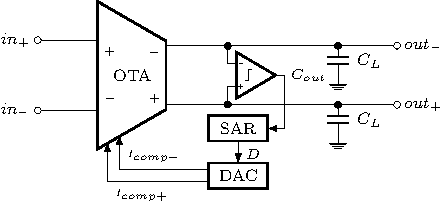
\includegraphics[scale=1]{fdota.pdf}\\
\end{center}
\caption 
{ \label{fig:fdota} 
Schemat blokowy FDOTA z cyfrową kalibracją napięcia niezrównoważenia.}
\end{figure}
\begin{figure}[!h]
  \begin{center}
  	\setlength{\tabcolsep}{0pt}
  	\begin{tabular}{ll}
  		(a) & (b)\\
  		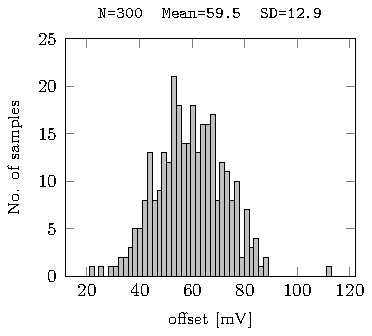
\includegraphics[height=5.2cm]{hist1.pdf}&
  		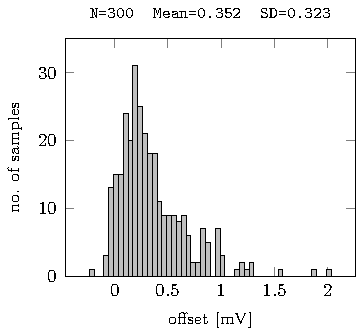
\includegraphics[height=5.2cm]{hist2.pdf}\\
  	\end{tabular}
  \end{center}
\caption
{ \label{fig:otah1} 
Rozrzut napięcia niezrównoważenia FDOTA: (a) bez kalibracji, (b) z 9-bitową kalibracją.}
\end{figure} 


\pagebreak


\section{Składanie wzorów}
\label{sec:wzory}
Jedną z wielu zalet {\LaTeX}-a, jak przystało na system składu publikacji naukowych, jest tryb matematyczny. W tym podrozdziale pokazano szereg przykładów użycia podstawowych konstrukcji tego trybu.

\subsection{Formuły w osobnych wierszach}
Podstawowym sposobem składania wzorów jest umieszczanie ich w osobnym wierszu. Wzory powinny być numerowane, tak jak to widać w poniższy przykładzie:
\begin{equation}
y= \frac{x-1}{x+2} 
\end{equation}
Automatyczną numerację uzyskujemy stosując otoczenie \texttt{\textbackslash begin\{equation\}\dots\textbackslash end\{equation\}}.
Umieszczenie etykiety umożliwi łatwe odwoływanie się do wzoru w~tekście, np. do formuły \ref{Eq:frac}.

\subsection{Formuły osadzone w tekście}
W najprostszym przypadku wzory mogą być integralną częścią akapitu, np. $E=mc^2$. Trzeba jednak pamiętać, że takie rozwiązanie stosujemy tylko do bardzo prostych (pomocniczych) zależności. Taka formuła jest trudna do odnalezienia, nie można uzyskać do niej odsyłacza a jeśli jest bardziej rozbudowana "rozpycha" tekst.

Szczególnie niekorzystnie  prezentują się osadzone w tekście ułamki ze względu na zmniejszony stopień pisma,  np. $y= \frac{x-1}{x+2}$. Jeśli zdecydujemy się temu zaradzić stosując polecenie \texttt{dfrac} zamiast \texttt{frac}, np.:  $y=\dfrac{x-1}{x+2}$, to znacząco zaburzona zostanie wielkość odstępów międzywierszowych, przez co tekst prezentuje się w sposób mało profesjonalny.

\subsection{Ułamki z ukośnikiem}
Proste ułamki lub miana można zapisać z wykorzystaniem ukośnika, np.: $\sfrac{1}{3}$, $\sfrac{1}{n}$, $\sfrac{V}{A}$.



\subsection{Indeksy górne i dolne}
Często spotykane są wyrażenia, w których stosowane są indeksy górne i dolne, np.:
\begin{equation}
a_{1},\ a_{i_{1}},\ a^{2},\ a^{b^{c}},\ a^{i_{1}},\
a_{i} + 1,\ a_{i + 1},\ a_{2}^{1},\ a^{2}_{1}
\end{equation}


\begin{equation}
x_{1} + x_{2} + \dots + x_{n}
\end{equation}


\subsection{Nawiasy i ograniczniki}
Szereg symboli takich jak nawiasy występuje w kilku odmianach różniących się wielkością. np.:
\[
( \dots \big( \dots \Big( \dots \bigg( \dots \Bigg(
\]
Zastosowanie "dużych" symboli poprawia czytelność złożonych formuł, np.: 
\[
F(x) |^{b}_{a} \dots
F(x) \bigr|^{b}_{a} \dots
F(x) \Bigr|^{b}_{a}
\]

\[
[ \sum_i a_i ]^{1/p} \dots  \left[ \sum_i a_i \right]^{1/p} \dots  \bigg[ \sum_i a_i \bigg]^{1/p} \dots  \Bigg[ \sum_i a_i \Bigg]^{1/p}
\]


\section{Ułamki piętrowe}

Zastosowanie zwykłego polecenia \texttt{frac} nie daje dobrych rezultatów:
\begin{equation}
  x = a_0 + \frac{1}{a_1
          + \frac{1}{a_2
          + \frac{1}{a_3 + \frac{1}{a_4} } } }
\end{equation}
W takiej sytuacji należy zastosować instrukcję \texttt{cfrac}:
\begin{equation}
  x = a_0 + \cfrac{1}{a_1
          + \cfrac{1}{a_2
          + \cfrac{1}{a_3 + \cfrac{1}{a_4} } } }
\end{equation}

\section{Justowanie wzorów}
Jeśli w tekście występuje kolejno kilka formuł to powinny one być wyjustowane względem siebie. Efekt ten uzyskuje się za pomocą otoczenia \texttt{\textbackslash begin\{align\}\dots\textbackslash end\{align\}}. W~formułach umieszczany jest symbol "\&", którego położenie wyznacza punkt odniesienia w każdej z~nich. Poniżej kilka przykładów wyjustowanych formuł.
\begin{align}
r^{2} &= s^{2} + t^{2}, \label{Eq:Pyth}\\
2u + 1 &= v + w^{\alpha}, \label{Eq:alpha}\\
x &= \frac{y + z}{\sqrt{s + 2u}};\label{Eq:frac}
\end{align}
\begin{align}
h(x) &= \int \left( \frac{f(x) + g(x)}{1+ f^{2}(x)} + \frac{1+ f(x)g(x)}{\sqrt{1 - \sin x}} \right) \, dx\label{E:longInt}=\\
&= \int \frac{1 + f(x)}{1 + g(x) } \, dx - 2 \tan^{-1}(x-2)\notag
\end{align}
W niektórych przypadkach samo justowanie nie wystarcza, np. podczas składania wzoru funkcji określonej przedziałami. W takim przypadku korzystamy z otoczenia \texttt{\textbackslash begin\{cases\}\dots \textbackslash end\{cases\}}. 
\begin{equation}
f(x)=
\begin{cases}
-x^{2}, &\text{if $x < 0$;}\\
\alpha + x, &\text{if $0 \leq x \leq 1$;}\\
x^{2}, &\text{otherwise.}
\end{cases}
\end{equation}



\section{Ingerowanie w skład dokumentu}
{\LaTeX} stara się rozmieścić tekst i inne elementy takie jak tabele, ilustracje czy wzory tak, aby uzyskać najlepszy efekt. Zdarza się jednak, np. kiedy blisko siebie występuje  duża liczba rysunków, że trzeba zaingerować  w układ pracy. 
\subsection{Kotwiczenie rysunków i tabel}
Jedną z najczęściej spotkanych sytuacji jest wymuszenie konkretnej pozycji ilustracji lub tabeli. W~tym celu należy definicję obiektu, czyli otoczenie \texttt{table} lub \texttt{figure}, uzupełnić o opcje wskazujące pożądaną lokalizację obiektu: \texttt{\textbackslash begin\{table\}\textbf{[!h]}},	\texttt{\textbackslash begin\{figure\}\textbf{[!h]}}. Litera \textit{h} jest skrótem od \textit{here}. Wykrzyknik nakazuje zaniechanie stosowania standardowych reguł rozmieszczania rysunków i tabel.

\subsection{Wymuszanie złamania strony}
Można wymusić złamanie strony w~konkretnym miejscu wstawiając polecenie  \texttt{\textbackslash pagebreak[\textit{n}]} (gdzie opcjonalny parametr \textit{n}=1\dots 4), które  {\LaTeX} interpretuje jako życzenie by zakończyć w tym miejscu stronę, tym silniejsze im większa jest wartość \textit{n}. 

\subsection{Wymuszanie złamania wiersza}
W celu wymuszenia przejścia do nowego wiersza \textit{bez rozpoczynania nowego akapitu} można zastosować polecenie \texttt{\textbackslash\textbackslash} lub \texttt{\textbackslash newline}.

\subsection{Zapobieganie wstawianiu wcięcia akapitowego}
Czasem (np. w sytuacji cytowania w podrozdziale \ref{fonty}) chcemy wstawić wiersz odstępu i jednocześnie uniknąć rozpoczęcia nowego akapitu. Wtedy na początku bloku tekstu wstawiamy polecenie \texttt{\textbackslash noindent}.

\subsection{Zapobieganiu przenoszeniu do nowego wiersza}
{\LaTeX} składając akapity stosuje automatyczne dzielenie i przenoszenie wyrazów, zgodnie z~regułami obowiązującymi w~języku, w jakim tworzony jest dokument. Zdarza się niekiedy, że zostaje rozdzielony   w ten sposób tekst, którego nie chcemy dzielić, np.: adres internetowy, stała fizyczna, itp. Można zapobiec dzieleniu słów i~przenoszeniu do nowego wiersza umieszczając tekst jako argument polecenia  \texttt{\textbackslash mbox\{\dots \}}. Poniżej przykład takiej sytuacji.
\vskip12pt
\textit{TeXstudio} jest dostępne nieodpłatnie na wszystkie platformy systemowe  na \url{http://texstudio.sourceforge.net/}.
\vskip12pt
\textit{TeXstudio} jest dostępne nieodpłatnie na wszystkie platformy systemowe  na \mbox{\url{http://texstudio.sourceforge.net/}}.

\subsection{Znaki specjalne}
Zdarza się że, musimy użyć słowa, które zawiera znak specjalny {\LaTeX}-a. Przykładem takiej sytuacji jest cytowanie nazwy pliku, która zawiera znak podkreślenia  "\_", np. w nazwie pliku \textit{praca\_dyplomowa.tex}. Wtedy należy taki znak poprzedzić odwróconym ukośnikiem czy znakiem \textbackslash.

\newpage
\section{Spis literatury}
Spis literatury generowany jest automatycznie, na podstawie umieszczonych w tekście odsyłaczy do rekordów bazy bibliograficznej.  
\subsection{Baza bibliograficzna w formacie \BibTeX}
Baza bibliograficzna w formacie \BibTeX jest w istocie plikiem tekstowym (o nazwie zwyczajowo zakończonej przez rozszerzenie \texttt{.bib}) zawierającym rekordy opisujące poszczególne pozycje. Praktycznie wszystkie wydawnictwa dostarczają referencji w formacie  \BibTeX, tak więc skompletowanie odpowiednio sformatowanej bazy bibliograficznej nie będzie nastręczało żadnych trudności. Każdy rekord w bazie musi zawierać  identyfikujący go unikalny klucz (etykietę). W podanym poniżej przykładzie są to \texttt{Pastre2006}, \texttt{Pastre2009}, \texttt{Pelgrom1989} i \texttt{wikibook}. 

{\footnotesize \begin{verbatim} 
@BOOK{Pastre2006,
  author = {Marc Pastre and Maher Kayal},
  title = {Methodology for the Digital Calibration of Analog Circuits and Systems: with 
  Case Studies (The Springer International Series in Engineering and Computer Science)},
  year = {2006},
  publisher = {Springer},
  isbn = {1402042523},
  url = {http://www.amazon.com/Methodology-Digital-Calibration-Circuits-Systems/dp/}
}
@INPROCEEDINGS{Pastre2009,
  author = {Pastre, M. and Kayal, M.},
  title = {Methodology for the digital calibration of analog circuits and systems 
  using sub-binary radix DACs},
  booktitle = {Mixed Design of Integrated Circuits Systems, 2009. MIXDES '09. MIXDES-16th
  International Conference},
  year = {2009},
  pages = {456-461},
  keywords = {analogue integrated circuits;calibrationy}
}
@ARTICLE{Pelgrom1989,
  author = {Pelgrom, M. J M and Duinmaijer, Aad C J and Welbers, A.P.G.},
  title = {Matching properties of MOS transistors},
  year = {1989},
  volume = {24},
  number = {5},
  pages = {1433-1439},
  issn = {0018-9200},
  journal = {Solid-State Circuits, IEEE Journal of},
  keywords = {MOS integrated circuits;insulated gate field effect transistors}
}
@WWW{wikibook,
  author = {Wikibooks},
  title = {LaTeX -- Wikibooks{,} The Free Textbook Project},
  year = {2012},
  url = {http://en.wikibooks.org/wiki/LaTeX}
}
\end{verbatim}
}

Bazę bibliograficzną można przygotować przy pomocy dowolnego edytora tekstowego lub specjalnego programu, np. \textit{JabRef} (\url{http://www.jabref.org/}).

\subsection{Odsyłacze}
W celu umieszczenia w tekście odsyłacza do konkretnej pozycji (lub grupy pozycji) należy użyć polecenia \texttt{\textbackslash cite\{klucz1,klucz2,\ldots \}}. Przykładowo,  umieszczenie w jednym miejscu odsyłaczy do dwóch pozycji wygląda następująco: \texttt{\textbackslash cite\{Pastre2006,Pelgrom1989\}}, co po przetworzeniu  da następujący efekt: \cite{Pastre2006,Pelgrom1989}. W przypadku sekwencji trzech odsyłaczy do kolejnych pozycji \texttt{\textbackslash cite\{Pastre2006,Pastre2009,Pelgrom1989\}}  efektem będzie \cite{Pastre2006,Pastre2009,Pelgrom1989}. W tym drugim przypadku wykryta została sekwencja odsyłaczy do  kolejnych pozycji literatury i automatycznie zastąpiono ją przedziałem indeksów. 

\subsection{Generowanie spisu literatury}
Wygenerowanie spisu literatury wymaga kilku przebiegów kompilatora (np. \texttt{pdflatex}, \texttt{lualatex}). Wynika to z faktu, że w trakcie przetwarzania  tekstu nie są jeszcze znane wszystkie odwołania do pozycji bibliografii. 

Po każdym przebiegu kompilatora tworzony jest pomocniczy plik (o rozszerzeniu \texttt{.aux}) zawierający klucze cytowanych pozycji. Dopiero na tej podstawie specjalny program \texttt{bibtex} może wygenerować zestawienie cytowanych pozycji bibliografii (plik z rozszerzeniem \texttt{.bbl}). To zestawienie jest wykorzystywane w kolejnym przebiegu kompilatora do wygenerowania rozdziału \textit{Bibliografia} w miejscu, w którym tekst zawiera polecenie \texttt{\textbackslash bibliography\{nazwa\_bazy\_bibliograficznej\}} oraz zastąpienia odsyłaczy identyfikatorami. Postać identyfikatorów zależy od przyjęto stylu formatowania bibliografii. W tym dokumencie zastosowany najprostszy styl czyli oznaczenie kolejnych pozycji spisu literatury kolejnymi liczbami (polecenie \texttt{\textbackslash bibliographystyle\{plainurl\}}).

Taka procedura całkowicie uwalnia użytkownika od konieczności samodzielnego wstawiania indeksów oraz bardzo kłopotliwego i podatnego na błędy korygowania tych indeksów po każdej modyfikacji bazy bibliograficznej.    

Znacznym ułatwieniem w tej sytuacji jest zastosowanie "inteligentnego" środowiska (np. \mbox{\textit{TeXStudio}}), które samodzielnie wywołuje w poprawnej kolejności wszystkie niezbędne programy w celu wygenerowania aktualnego zestawienia bibliografii. 

Jeśli zajdzie potrzeba wymuszenia ponownej generacji bibliografii należy usunąć plik \texttt{.bbl} oraz zaktualizować datę modyfikacji bazy bibliograficznej a następnie  uruchomić przetwarzanie dokumentu.




%%%%%%%%%%%%%%%%%%%%%%%%%%%%%%%%%%%%%%%%%%%%%%%%%%%%%%%%%%%%%%%%%%%%%%%%%%%%%%%%%%%%%%%%%
%%%%%%%%%%%%%%%%%%%%%%%%%%%%%%%%%%%%%%%%%%%%%%%%%%%%%%%%%%%%%%%%%%%%%%%%%%%%%%%%%%%%%%%%%
\end{verbatim}
}

\subsection{Ilustracje}
Zakłada się, że pliki graficzne zawierające ilustracje są umieszczone w katalogu \textit{grafika}.

\subsection{Bibliografia}
Zakłada się, że baza bibliograficzna znajduje się w  pliku o nazwie \textit{spis.bib}  a sam plik w~podkatalogu \textit{bibliografia} co znajduje swoje odzwierciedlenie w poleceniu:

{\footnotesize \begin{verbatim}
\bibliography{../bibliografia/spis}
\end{verbatim}
}



\chapter{Uwagi ogólne}
 

\section{Typografia}
\textit{Typografia to dziedzina grafiki użytkowej obejmująca ukształtowanie i układ elementów graficznych drukowanych publikacji}. Zasady rządzące układem tekstu i~innych składników dzieła są określone przez Polską Normę \cite{PN}. Należy zaznaczyć, że przestrzeganie zasad typografii jest równie ważne jak poprawność pod względem gramatycznym i~ortograficznym.

Ocena pracy dyplomowej zależy w dużej mierze od wrażenia jakie odnosi recenzent. Usterki takie jak chaotyczny układ treści, nieczytelne rysunki, źle sformatowane wzory, niekonsekwentne justowanie akapitów, itd.  odbiją się z pewnością negatywnie na odbiorze pracy. 


 

\section{Poprawność językowa}
Praca dyplomowa musi być poprawna pod względem językowym. Celem tego dokumentu nie jest przypominanie zasad gramatyki i ortografii ani nauczanie poprawnego stylu. Tę~wiedzę dyplomanci już posiedli o~czym świadczy pozytywny wynik egzaminu dojrzałości. Jednak często okazuje się, że stosowanie tej wiedzy w praktyce sprawia znaczne trudności. Usterki, które najczęściej występują w~pracach dyplomowych a~zarazem są szczególnie irytujące to:
\begin{itemize}
\item błędy interpunkcyjne (zwłaszcza brak lub nadmiar przecinków),
\item pisownia łączna cząstek \emph{-bym}, \emph{-byś}, \emph{-by}, \emph{-byśmy}, \emph{-byście},
\item pisownia rozdzielna cząstek \emph{bym}, \emph{byś}, \emph{by}, \emph{byśmy}, \emph{byście},
\item pisownia łączna i rozdzielna partykuły \emph{nie}, 
\item stosowanie skrótów myślowych, kolokwializmów i żargonu,
\item nadużywanie strony biernej.
\end{itemize}
Jeśli pojawiają się wątpliwości natury językowej należy sięgać do słowników. Szczególnie godne polecenia są: \emph{Wielki słownik ortograficzny PWN} oraz \emph{Wielki słownik poprawnej polszczyzny PWN}. Natychmiastową pomocą służą też internetowe poradnie językowe, np. \url{http://poradnia.pwn.pl/}. 

Warto też pamiętać, że zastosowanie programów do weryfikacji ortografii nie zawsze ustrzeże autora przed błędami. Często popełniony błąd -- tzw. literówka -- powoduje, że powstaje poprawne słowo, ale o~innym znaczeniu, np. \textit{też} i \textit{tez},  \textit{tez} i \textit{łez}, \emph{dla} i \emph{dal}, \textit{układu} i~\textit{układy}, \textit{jaka} i \textit{jaką}, itp.


\section{Wydruk czarno-biały czy kolorowy?}
Przed przystąpieniem do edycji pracy dyplomowej należy podjąć decyzję czy wydruk będzie kolorowy czy czarno-biały. Decyzja ta wpływa na sposób wykonania ilustracji: diagramów, schematów blokowych, wykresów, zrzutów ekranowych, itd. Przygotowanie ilustracji jest czasochłonne a~zmiana decyzji w~trakcie edycji będzie wymagać daleko idących modyfikacji.

Należy pamiętać, że odwzorowanie kolorów na ekranie monitora jest inne niż  na wydruku. Profesjonalne edytory graficzne pozwalają uwzględnić te różnice o ile znane są profile monitora i drukarki a urządzenia te są poprawnie skalibrowane. Zwykle jednak do edycji prac dyplomowych narzędzia takie nie są wykorzystywane i dlatego konieczne jest wykonanie próbnych wydruków w~celu ustalenia odpowiedniej palety i~nasycenia kolorów.

\section{Dobór narzędzi}
\label{sec:tools}
\subsection{System składu {\LaTeX}}
Zastosowanie  {\LaTeX}-a uwalnia  autora od problemów definiowania stylów, doboru stopnia pisma tekstu, tytułów rozdziałów, poprawnego numerowania rysunków, tabel i~wzorów, itd. Co istotne, {\LaTeX}  jest bezpłatny i~jest dostępny na wszystkich popularnych platformach systemowych (Linux, Windows, Mac OS). 

Przed przystąpieniem do edycji pracy dyplomowej niezbędne będzie zainstalowanie aktualnej dystrybucji systemu  {\LaTeX}. Autor tego opracowania zaleca dystrybucję \textit{TeX Live}, dostępną na wszystkie platformy systemowe. Jej zastosowanie gwarantuje bezproblemowe przenoszenie tekstu pracy pomiędzy komputerami z różnymi systemami operacyjnymi. Można ją pobrać z serwera o adresie \url{https://www.tug.org/texlive/}.

\subsection{Edytor tekstu}
Należy pamiętać, że {\LaTeX} nie jest procesorem tekstu a systemem składu. Najtrafniejsze jest porównanie go do kompilatora. Zatem pliki źródłowe można przygotować  za pomocą dowolnego edytora tekstowego, który pozwoli tworzyć dokumenty z~kodowaniem znaków UTF-8. Jednak znacznie wygodniej jest wykorzystać jedno z wielu dostępnych środowisk zaprojektowanych specjalnie do edycji dokumentów  {\LaTeX}. W opinii autora tego dokumentu jednym z najlepszych narzędzi tego typu jest  \textit{TeXstudio} dostępne nieodpłatnie na wszystkich popularnych platformach systemowych (\url{http://texstudio.sourceforge.net/}).

\subsection{Ilustracje}
Oprócz edytora tekstowego niezbędne będą programy do tworzenia grafiki rastrowej i~wektorowej. Posłużą one do przetworzenia zrzutów ekranowych czy też wykresów przedstawiających wyniki symulacji a~także przygotowania diagramów i schematów blokowych. Można wykorzystać dowolne narzędzia o ile pozwolą one na zapisanie (wyeksportowanie) plików graficznych w formatach takich jak PDF czy PNG. Więcej informacji na temat przygotowywanie ilustracji znajduje się w rozdziale \ref{sec:ilustracje}.
 
\subsection{Wybór fontu}
Na potrzeby pracy dyplomowej  wystarczy stosować fonty zawarte w standardowej instalacji systemu {\LaTeX} (np. dystrybucji \textit{TeX Live}). Jedynym wyjątkiem jest  stosowany na stronie tytułowej font \textit{Belgrano} (licencja \textit{SIL Open Font License}), który znajduje się w podkatalogu \textit{./fonts} i który należy zainstalować  przy pomocy standardowych narzędzi dostępnych w~konkretnym systemie operacyjnym.

Niniejszy dokument złożony jest fontem \textit{FreeSerif}, który należy do rodziny \textit{GNU FreeFont}. Jego zaletą jest to, że pozwala uzyskać czytelny a jednocześnie zwarty tekst. Domyślny font jest zdefiniowany przy pomocy polecenia \texttt{\textbackslash setmainfont\{\}}), jak w cytowanym poniżej fragmencie głównego pliku:

{\footnotesize \begin{verbatim}
%%%%%%%%%%%%%%%%%%%%%%%%%%%%%%%%%%%%%%%%%%%%%%%%%%%%%%%%%%%%%%%%%%%%%%%%%%%%%%%%%%%%%%%%%
%%% Konfiguracja fontu
%%%\setmainfont{TeX Gyre Pagella}
\setmainfont{FreeSerif}
%%%%%%%%%%%%%%%%%%%%%%%%%%%%%%%%%%%%%%%%%%%%%%%%%%%%%%%%%%%%%%%%%%%%%%%%%%%%%%%%%%%%%%%%%
\end{verbatim}
}

\noindent Font \textit{FreeSerif} powinien znajdować się w standardowej dystrybucji  {\LaTeX}-a. Jeśli z jakiegoś powodu nie jest dostępny można go pobrać np. z serwerów \url{http://www.fontspace.com/gnu-freefont/freeserif} lub \url{https://www.gnu.org/software/freefont/}\ . Po pobraniu plików fonty należy zainstalować  przy pomocy standardowych narzędzi dostępnych w~konkretnym systemie operacyjnym. Trzeba pamiętać o~zainstalowaniu wszystkich odmian tzn.: \textit{regular}, \textit{bold}, \textit{italic}, \textit{bolditalic}, itd. 

Jeśli w dokumencie brak jest polecenia \texttt{\textbackslash setmainfont\{\}} to zastosowany będzie font \textit{Latin Modern Roman}, o bardzo charakterystycznym wyglądzie. Poniżej przykład akapitu złożonego z wykorzystaniem tego fontu:

\vskip18pt
\noindent\parbox{\textwidth}{
\setmainfont{Latin Modern Roman}
Lorem ipsum dolor sit amet enim. Etiam ullamcorper. Suspendisse a pellentesque dui, non felis. Maecenas malesuada elit lectus felis, malesuada ultricies. Curabitur et ligula. Ut molestie a, ultricies porta urna. Vestibulum commodo volutpat a, convallis ac, laoreet enim. Phasellus fermentum in, dolor. Pellentesque facilisis. Nulla imperdiet sit amet magna. Vestibulum dapibus, mauris nec malesuada fames ac turpis velit, rhoncus eu, luctus et interdum adipiscing wisi. }
\vskip18pt
\noindent Jeśli zastosujemy polecenie \texttt{\textbackslash setmainfont\{TeX Gyre Pagella\}} to uzyskamy tekst o następującym wyglądzie:
\vskip18pt
\noindent\parbox{\textwidth}{
\setmainfont{TeX Gyre Pagella}
Lorem ipsum dolor sit amet enim. Etiam ullamcorper. Suspendisse a pellentesque dui, non felis. Maecenas malesuada elit lectus felis, malesuada ultricies. Curabitur et ligula. Ut molestie a, ultricies porta urna. Vestibulum commodo volutpat a, convallis ac, laoreet enim. Phasellus fermentum in, dolor. Pellentesque facilisis. Nulla imperdiet sit amet magna. Vestibulum dapibus, mauris nec malesuada fames ac turpis velit, rhoncus eu, luctus et interdum adipiscing wisi.}\label{fonty}

\vskip18pt



% !TeX encoding = UTF-8
% !TeX spellcheck = pl_PL
\chapter{Wskazówki i przykłady}

W rozdziale tym zamieszczono szereg wskazówek i przykładów formatowania  w~{\LaTeX}-u typowych elementów pracy dyplomowej. Tekst źródłowy przykładów można skopiować i~przystosować do własnych potrzeb.

\section{Formatowanie tekstu}
\subsection{Font, style, itd.}
Font, stopień pisma tekstu i tytułów rozdziałów, wielkość wcięć i odstępów, itd. ustala sam {\LaTeX} na podstawie definicji zawartych w szablonie dokumentu. Użytkownik nie musi niczego definiować samodzielnie.

\subsection{Akapity}
Akapit nie wymaga  specjalnego formatowania. Tekst należy wpisywać bez wymuszania przejścia do nowego wiersza czyli tzw. ręcznego wstawiania znaków powrotu karetki. Liczba                       odstępów                        pomiędzy wyrazami,              tzw. \textit{spacji},   większa niż jeden jest  interpretowana jak jeden odstęp.

W celu rozpoczęcia  nowego akapitu należy pozostawić wiersz odstępu. Wszystkie parametry tekstu takie jak wcięcia akapitowe, odstępy między wierszami i~między akapitami  ustawia sam  {\LaTeX}. 

Należy pamiętać, aby nie pozostawiać na końcu wiersza samotnego spójnika (np.:~"i", "a", "z").  W tym celu pomiędzy spójnik i następny wyraz należy wstawić tzw. "niełamliwy" odstęp. W  \mbox{{\LaTeX}-u} uzyskuje się taki odstęp przez umieszczenie pomiędzy wyrazami znaku "\textasciitilde" zamiast zwykłego odstępu, np. "w\textasciitilde tekście".


\subsection{Wstawianie specjalnych symboli}
Obecnie, dzięki pakietom językowym, nie ma potrzeby stosowania tzw. \textit{escape codes}  w celu uzyskania znaków narodowych (np.  \texttt{\textbackslash k\{a\}} dla uzyskania ą). Wystarczy zapisać tekst w pliku z kodowaniem UTF-8 oraz użyć odpowiedniego pakietu, np:
{\footnotesize \begin{verbatim}
\usepackage{polyglossia}
\setdefaultlanguage[]{polish}
\end{verbatim}
}

Często zachodzi potrzeba wstawienia symbolu, np. litery z greckiego alfabetu. Rozwiązanie tego problemu zależy od tego w jakim elemencie tekstu chcemy uzyskać taki symbol. 

Jeśli symbol występuje we wzorze to rozwiązaniem jest zastosowanie trybu matematycznego  (szczegóły w rozdziale \ref{sec:wzory}), w którym pożądany symbol wstawiamy za pomocą specjalnego kodu, np.: \texttt{\textbackslash mu} -- $\mu $, \texttt{\textbackslash pi}~--~$\pi$.

Jeśli symbol jest nazwą jednostki to wtedy można "awaryjnie" zastosować tryb matematyczny. Powstaje formuła osadzona w tekście, np. 3~$\mu m$. Jednak znacznie lepiej jest zastosować specjalne polecenia z pakietu \texttt{siunitx} uzyskując napis \SI{3}{\micro\meter}. Szczegóły w rozdziale \ref{sec:liczby}.

\subsection{Wyróżnianie tekstu}
W celu wyróżnienia fragmentu tekstu można zastosować \textit{specjalną odmianę  kroju czcionki zwaną italikiem}, \textbf{wytłuszczenie}  lub  \underline{podkreślenie}. Należy pamiętać, żeby nie nadużywać tej formy ekspresji. Zaleca się wybranie jednej z~tych metod wyróżniania tekstu i  konsekwentne jej stosowanie w całej pracy. Wytłuszczenia są często zarezerwowane dla oznaczania wektorów, macierzy, itd. Dlatego zwykłe wyróżnienie tekstu najlepiej zrealizować   \textit{przez zastosowanie italików}. 




\subsection{Wyliczenia}
Wyliczenia, zwane też listami, tworzymy korzystając  z otoczeń (ang.~\textit{environments}). {\LaTeX}  formatuje listy całkowicie automatycznie.  Najczęściej stosuje się dwa rodzaje list:
\begin{itemize}
\item \textit{nieuporządkowaną}, uzyskiwaną przez użycie otoczenia \texttt{itemize},
\item \textit{uporządkowaną}, uzyskiwaną przez użycie otoczenia \texttt{enumerate}.
\end{itemize}
Podczas składania list należy pamiętać o stosowaniu poprawnej interpunkcji. Poniżej dwa przykłady wyliczeń:
\begin{itemize}
\item Nieuporządkowana poziom pierwszy, 
\begin{itemize}
\item nieuporządkowana poziom drugi,
\begin{itemize}
\item nieuporządkowana poziom trzeci.
\end{itemize}
\end{itemize}
\end{itemize}

\begin{enumerate}
\item  Uporządkowana poziom pierwszy,
\begin{enumerate}
\item uporządkowana poziom drugi,
\begin{enumerate}
\item uporządkowana poziom trzeci.
\end{enumerate}
\end{enumerate}
\end{enumerate}




\subsection{Liczby}
\label{sec:liczby}
Liczby i miana należy sformatować zgodnie z zasadami typografii obowiązującymi w języku polskim oraz zgodnie z normami SI. Częstym błędem jest podawania wartości liczbowych w taki sposób w jaki wyświetlają je symulatory, np. 3.3V zamiast 3,3~V.  Należy zwrócić uwagę na stosowanie właściwego znaku oddzielającego część całkowitą od ułamkowej oraz na oddzielanie miana od samej liczby (najprostszym sposobem jest wstawienie pomiędzy liczbę i symbol tzw. niełamliwej spacji czyli tyldy). 

Problem formatowania liczb można rozwiązać w bardziej ogólny sposób używając pakietu \texttt{siunitx}.  Pakiet ten zawiera szereg poleceń, od prostych służących do formatowania liczb: \num{123e-5}, \ang{100}, \SI{1050}{\degreeCelsius}, \SI{1}{\micro\meter} aż po bardziej złożone służące do justowania liczb w tabelach.
\begin{table}[!h]
\caption{Przykład wykorzystania pakietu \texttt{siunitx} do justowania zawartości pól tabeli.}
\centering
  \begin{tabular}{@{}lS[table-format=3.2]>{\bfseries}S[table-format=3.2]@{}}
    \toprule
    \textbf{Foo} & \textbf{Normal} & \textbf{Bold} \\
    \midrule
    foo1 & 111 & 111 \\
    foo2 & 222.2 & 222.2 \\
    foo3 & 3.33 & 3.33 \\
    foo4 & 4 & 4 \\
    foo5 & 5.5 & 5.5 \\
    \bottomrule
  \end{tabular}
\end{table}


\subsection{Adresy internetowe}
Adresy internetowe formatujemy za pomocą polecenia \textbackslash url\{\textit{adres}\}, np. \url{http://www.tug.org/}.

\section{Przypisy}
Jeśli trzeba utworzyć przypis to w {\LaTeX}-u\footnote{{\LaTeX} - (od [Leslie] Lamport {\TeX}) oprogramowanie do zautomatyzowanego składu tekstu.}  korzystamy z instrukcji \texttt{ \textbackslash footnote\{\textit{przypis}\}}.

\section{Odsyłacze}
W tekście pracy dyplomowej często umieszcza się odniesienia do ilustracji, tabel, wzorów lub podrozdziałów.  {\LaTeX} sam zajmuje się generacją numeracji tych elementów. Tak więc na etapie tworzenia tekstu konkretne indeksy nie są jeszcze znane. Dlatego w tekście wstawia się odsyłacze do etykiet a same etykiety umieszcza w definicjach elementów, do których zamierzamy się odnosić.

Etykietę tworzy się za pomocą polecenia \texttt{\textbackslash label\{\textit{etykieta}\}}. Warto przemyśleć system tworzenia nazw etykiet tak, aby łatwo kojarzyły się z typem obiektu. Przykładowo, etykieta ilustracji zawiera prefiks \textit{fig:} (np. \textbackslash label\{fig:fdota\}) a ~etykieta wzoru  prefiks \textit{Eq:} (np. \textbackslash label\{Eq:ulamek\}). 

Odsyłacz powstaje poprzez umieszczenie polecenia \texttt{\textbackslash ref\{\textit{etykieta}\}} (np.~\textbackslash ref\{fig:fdota\}). A~oto przykłady zastosowania odsyłacza do rysunku: Rys.~\ref{fig:fdota}, wzoru  \ref{Eq:frac} i rozdziału \ref{sec:wzory}.

\section{Tabele}
Tabele składamy korzystając z otoczenia \texttt{tabular}. Podstawowe zasady składania tabel są proste i ich zastosowanie w praktyce nie powinno sprawiać trudności.  Jednak w przypadkach bardziej złożonych struktur (np. łączenie pól, kolumn, wierszy) czy też tabel wykraczających poza jedną stronę może się okazać, że konieczne będzie zastosowanie specjalnych pakietów {\LaTeX}-a. Przedstawienie zaawansowanych metod składania tabel wykracza poza zakres tego dokumentu. Zainteresowanych odsyłam do dokumentacji. Zawsze warto skorzystać ze wsparcia jakiego w tym zakresie udzielają wyspecjalizowane narzędzia na przykład wspominany już w~rozdziale~\ref{sec:tools} program \mbox{\textit{TeXstudio}}.     
\begin{table}[!h]
\caption{Przykładowa tabela -- zawartość pól wyśrodkowana.}
\centering
\begin{tabular}{|c||c|c|c|c|}
\hline & Nagłówek 1  & Nagłówek 2  & Nagłówek 3  &  Nagłówek 4 \\ 
\hline
\hline  Etykieta wiersza & bb bb bbbb bbbb  & cc  & dd   &  ee  \\
\hline  Etykieta wiersza & bb  & cc  & dd   &  ee \\
\hline  Etykieta wiersza  & bb  & cc  & dd   &  ee \\ 
\hline  Etykieta wiersza  & bb  & cc  & dd   &  ee ee eeee  eeeee\\
\hline 
\end{tabular} 
\label{tab:tab2}
\end{table}

\begin{table}[!h]
\caption{Przykładowa tabela -- wyrównywanie zawartości pól do lewego lub prawego  marginesu.}
\centering
\begin{tabular}{|l|l|r|}
\hline  Nagłówek 1  &  Nagłówek 2  &  Nagłówek 3  \\ 
\hline
\hline  bb bb bbbb bbbb   & dd   &  ee  \\
\hline   cc  & dd   &  ee ee eeee  eeeee\\
\hline 
\end{tabular} 
\label{tab:tab3}
\end{table}

\begin{table}[!h]
\centering
\caption{Przykład tabeli z diagonalnym podziałem komórki.}
\label{tab:time}
\begin{tabular}{|c|c|c|}
\hline
\diagbox{Etykieta wierszy}{Etykieta kolumn}  &  Nagłówek 1  & Nagłówek 2\\
\hline Nagłówek 1  &  Nagłówek 2  &  Nagłówek 3 \\ 
\hline AAAAA AAAAA & BBBB BBB & CCCC CCCC \\
\hline AAAAAA & 2 & 3 \\
\hline
\end{tabular}
\label{tab:tabdiag}
\end{table}

\begin{table}[!h]
\caption{Wymuszenie konkretnych  szerokości kolumn.}
\centering
\begin{tabular}{|l|l|p{25mm}|l|p{3cm}|}
\hline & Nagłówek 1  & Nagłówek 2  & Nagłówek 3  &  Nagłówek 4  \\ 
\hline
\hline  Etykieta wiersza & bb  & cc  & dd   &  Podstawowe zasady składania tabel są proste i ich zastosowanie w praktyce nie powinno sprawiać trudności \\
\hline  Etykieta wiersza  & bb  & cc cc cccc cccccc  & dd   &  ee \\ 
\hline 
\end{tabular} 
\label{tab:tab1}
\end{table}


\newpage
\section{Cytowanie kodu źródłowego}
Cytując kod programu czy też modelu HDL najlepiej jest skorzystać z pakietu \texttt{listings}, który definiuje otoczenie  \texttt{\textbackslash begin\{lstlisting\}}\dots\texttt{ \textbackslash end\{lstlisting\}}. Pakiet ten pozwala na automatyczne wyróżnianie słów kluczowych szeregu języków  programowania i opisu sprzętu. Poniżej pokazano przykłady: modelu VHDL (wydruk~\ref{lst:latch}), modelu Verilog (wydruk~\ref{lst:adder}) oraz programu w języku C++(wydruk~\ref{lst:hello}).

  
\begin{lstlisting}[language=VHDL, caption={Przykładowy model VHDL}, label={lst:latch}]
entity latch is
port (sample: in std_logic;
count : in  std_logic_vector (0 to 7);
data:   out std_logic_vector (0 to 7));
end latch;

architecture behav of latch is     -- zatrzask
begin
process (sample, count)
begin
	if (sample = '1') then
		data <= count;
	end if;
end process;
end behav;
\end{lstlisting}



\begin{lstlisting}[language=Verilog, caption={Przykładowy model Verilog}, label={lst:adder}]
module add_carry_signed_final (
input signed [2:0] A,
input signed [2:0] B,
input carry_in,
output signed [3:0] Sum);

assign Sum = A + B + $signed({1'b0, carry_in});

endmodule
\end{lstlisting}


\begin{lstlisting}[language=c++, caption={Przykładowy program C++}, label={lst:hello}]
// 'Hello World!' program 

#include <iostream>

int main()
{
	std::cout << "Hello World!" << std::endl;
	return 0;
}
\end{lstlisting}



\section{Ilustracje}
\label{sec:ilustracje}
Ilustracje są pobierane z plików, przy  czym preferowany jest format PDF lub PNG.
\subsection{Przygotowanie ilustracji}
O ile to możliwe ilustracje powinny być przygotowane w~postaci wektorowej, przy pomocy niezależnego oprogramowania i zapisane w plikach o formacie PDF lub SVG (ten drugi wariant wymaga lepszej znajomości {\LaTeX}-a). Zaawansowani użytkownicy mogą wykorzystać pakiety TikZ i PGF (\url{http://sourceforge.net/projects/pgf/}). 

Jeśli ilustracja dostępna jest tylko w wersji rastrowej (np. plik graficzny zawierający przebiegi uzyskane w trakcie  symulacji) to należy użyć formatu pliku o~bezstratnej kompresji a~zastosowana rozdzielczość  nie może być mniejsza niż 300~dpi a najlepiej 600~dpi. 

\textit{Uwaga! Tzw. zrzuty ekranowe mają rozdzielczość taką jak obraz na ekranie monitora czyli zwykle mniej niż 100~dpi i nie prezentują się dobrze na wydrukach.}   

Przygotowując ilustracje trzeba pamiętać, że zastosowany w nich font i stopień pisma musi być zgodny z wyglądem tekstu. Stosujemy ten sam font co w tekście (lub jeśli to niemożliwe, inny o podobnym kroju) a~wielkość napisów powinna być nieco mniejsza niż w tekście (jeśli stopień pisma tekstu wynosi 11~pt to ilustracje mogą stosować np. 9~pt). Można też zastosować w ilustracjach  font  bezszeryfowy (takich jak np.~Arial). Niezależnie od tego jaką konwencję przyjmiemy należy \textit{stosować ją konsekwentnie do wszystkich ilustracji}.

Kolejna kwestia to fizyczny rozmiar ilustracji. Przygotowywana grafika powinna mieć takie fizyczne wymiary, aby w~trakcie włączania jej do dokumentu nie dokonywać skalowania. Skalowanie bardzo źle wpływa na czytelność grafiki rastrowej. Ponadto skalowanie zmienia grubość linii i wielkość napisów. Jeśli nie zastosuje się jednakowych zasad to może się okazać, że ilustracje nie prezentują się w jednolity sposób co sprawia fatalne wrażenie.

\subsection{Składanie ilustracji}
Ilustracje mogą być zamieszczane pojedynczo (Rys.~\ref{fig:fdota}) lub, jak pokazano na Rys.~\ref{fig:otah1},  obok siebie korzystając z otoczenia \texttt{tabular} (Rys.~\ref{fig:otah1}). Można też  zastosować polecenie \textbackslash \texttt{subfloat}.
\begin{figure}[!h]
\begin{center}
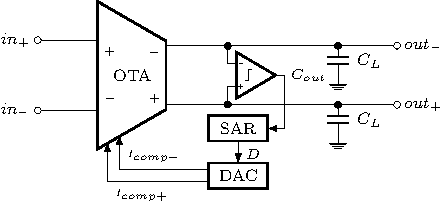
\includegraphics[scale=1]{fdota.pdf}\\
\end{center}
\caption 
{ \label{fig:fdota} 
Schemat blokowy FDOTA z cyfrową kalibracją napięcia niezrównoważenia.}
\end{figure}
\begin{figure}[!h]
  \begin{center}
  	\setlength{\tabcolsep}{0pt}
  	\begin{tabular}{ll}
  		(a) & (b)\\
  		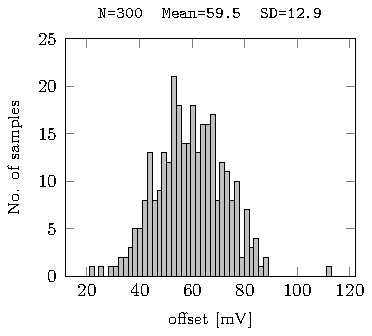
\includegraphics[height=5.2cm]{hist1.pdf}&
  		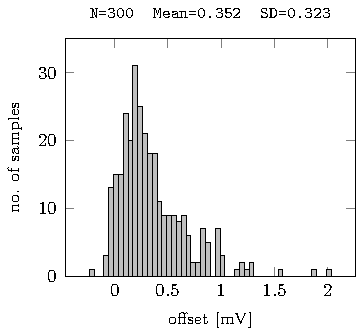
\includegraphics[height=5.2cm]{hist2.pdf}\\
  	\end{tabular}
  \end{center}
\caption
{ \label{fig:otah1} 
Rozrzut napięcia niezrównoważenia FDOTA: (a) bez kalibracji, (b) z 9-bitową kalibracją.}
\end{figure} 


\pagebreak


\section{Składanie wzorów}
\label{sec:wzory}
Jedną z wielu zalet {\LaTeX}-a, jak przystało na system składu publikacji naukowych, jest tryb matematyczny. W tym podrozdziale pokazano szereg przykładów użycia podstawowych konstrukcji tego trybu.

\subsection{Formuły w osobnych wierszach}
Podstawowym sposobem składania wzorów jest umieszczanie ich w osobnym wierszu. Wzory powinny być numerowane, tak jak to widać w poniższy przykładzie:
\begin{equation}
y= \frac{x-1}{x+2} 
\end{equation}
Automatyczną numerację uzyskujemy stosując otoczenie \texttt{\textbackslash begin\{equation\}\dots\textbackslash end\{equation\}}.
Umieszczenie etykiety umożliwi łatwe odwoływanie się do wzoru w~tekście, np. do formuły \ref{Eq:frac}.

\subsection{Formuły osadzone w tekście}
W najprostszym przypadku wzory mogą być integralną częścią akapitu, np. $E=mc^2$. Trzeba jednak pamiętać, że takie rozwiązanie stosujemy tylko do bardzo prostych (pomocniczych) zależności. Taka formuła jest trudna do odnalezienia, nie można uzyskać do niej odsyłacza a jeśli jest bardziej rozbudowana "rozpycha" tekst.

Szczególnie niekorzystnie  prezentują się osadzone w tekście ułamki ze względu na zmniejszony stopień pisma,  np. $y= \frac{x-1}{x+2}$. Jeśli zdecydujemy się temu zaradzić stosując polecenie \texttt{dfrac} zamiast \texttt{frac}, np.:  $y=\dfrac{x-1}{x+2}$, to znacząco zaburzona zostanie wielkość odstępów międzywierszowych, przez co tekst prezentuje się w sposób mało profesjonalny.

\subsection{Ułamki z ukośnikiem}
Proste ułamki lub miana można zapisać z wykorzystaniem ukośnika, np.: $\sfrac{1}{3}$, $\sfrac{1}{n}$, $\sfrac{V}{A}$.



\subsection{Indeksy górne i dolne}
Często spotykane są wyrażenia, w których stosowane są indeksy górne i dolne, np.:
\begin{equation}
a_{1},\ a_{i_{1}},\ a^{2},\ a^{b^{c}},\ a^{i_{1}},\
a_{i} + 1,\ a_{i + 1},\ a_{2}^{1},\ a^{2}_{1}
\end{equation}


\begin{equation}
x_{1} + x_{2} + \dots + x_{n}
\end{equation}


\subsection{Nawiasy i ograniczniki}
Szereg symboli takich jak nawiasy występuje w kilku odmianach różniących się wielkością. np.:
\[
( \dots \big( \dots \Big( \dots \bigg( \dots \Bigg(
\]
Zastosowanie "dużych" symboli poprawia czytelność złożonych formuł, np.: 
\[
F(x) |^{b}_{a} \dots
F(x) \bigr|^{b}_{a} \dots
F(x) \Bigr|^{b}_{a}
\]

\[
[ \sum_i a_i ]^{1/p} \dots  \left[ \sum_i a_i \right]^{1/p} \dots  \bigg[ \sum_i a_i \bigg]^{1/p} \dots  \Bigg[ \sum_i a_i \Bigg]^{1/p}
\]


\section{Ułamki piętrowe}

Zastosowanie zwykłego polecenia \texttt{frac} nie daje dobrych rezultatów:
\begin{equation}
  x = a_0 + \frac{1}{a_1
          + \frac{1}{a_2
          + \frac{1}{a_3 + \frac{1}{a_4} } } }
\end{equation}
W takiej sytuacji należy zastosować instrukcję \texttt{cfrac}:
\begin{equation}
  x = a_0 + \cfrac{1}{a_1
          + \cfrac{1}{a_2
          + \cfrac{1}{a_3 + \cfrac{1}{a_4} } } }
\end{equation}

\section{Justowanie wzorów}
Jeśli w tekście występuje kolejno kilka formuł to powinny one być wyjustowane względem siebie. Efekt ten uzyskuje się za pomocą otoczenia \texttt{\textbackslash begin\{align\}\dots\textbackslash end\{align\}}. W~formułach umieszczany jest symbol "\&", którego położenie wyznacza punkt odniesienia w każdej z~nich. Poniżej kilka przykładów wyjustowanych formuł.
\begin{align}
r^{2} &= s^{2} + t^{2}, \label{Eq:Pyth}\\
2u + 1 &= v + w^{\alpha}, \label{Eq:alpha}\\
x &= \frac{y + z}{\sqrt{s + 2u}};\label{Eq:frac}
\end{align}
\begin{align}
h(x) &= \int \left( \frac{f(x) + g(x)}{1+ f^{2}(x)} + \frac{1+ f(x)g(x)}{\sqrt{1 - \sin x}} \right) \, dx\label{E:longInt}=\\
&= \int \frac{1 + f(x)}{1 + g(x) } \, dx - 2 \tan^{-1}(x-2)\notag
\end{align}
W niektórych przypadkach samo justowanie nie wystarcza, np. podczas składania wzoru funkcji określonej przedziałami. W takim przypadku korzystamy z otoczenia \texttt{\textbackslash begin\{cases\}\dots \textbackslash end\{cases\}}. 
\begin{equation}
f(x)=
\begin{cases}
-x^{2}, &\text{if $x < 0$;}\\
\alpha + x, &\text{if $0 \leq x \leq 1$;}\\
x^{2}, &\text{otherwise.}
\end{cases}
\end{equation}



\section{Ingerowanie w skład dokumentu}
{\LaTeX} stara się rozmieścić tekst i inne elementy takie jak tabele, ilustracje czy wzory tak, aby uzyskać najlepszy efekt. Zdarza się jednak, np. kiedy blisko siebie występuje  duża liczba rysunków, że trzeba zaingerować  w układ pracy. 
\subsection{Kotwiczenie rysunków i tabel}
Jedną z najczęściej spotkanych sytuacji jest wymuszenie konkretnej pozycji ilustracji lub tabeli. W~tym celu należy definicję obiektu, czyli otoczenie \texttt{table} lub \texttt{figure}, uzupełnić o opcje wskazujące pożądaną lokalizację obiektu: \texttt{\textbackslash begin\{table\}\textbf{[!h]}},	\texttt{\textbackslash begin\{figure\}\textbf{[!h]}}. Litera \textit{h} jest skrótem od \textit{here}. Wykrzyknik nakazuje zaniechanie stosowania standardowych reguł rozmieszczania rysunków i tabel.

\subsection{Wymuszanie złamania strony}
Można wymusić złamanie strony w~konkretnym miejscu wstawiając polecenie  \texttt{\textbackslash pagebreak[\textit{n}]} (gdzie opcjonalny parametr \textit{n}=1\dots 4), które  {\LaTeX} interpretuje jako życzenie by zakończyć w tym miejscu stronę, tym silniejsze im większa jest wartość \textit{n}. 

\subsection{Wymuszanie złamania wiersza}
W celu wymuszenia przejścia do nowego wiersza \textit{bez rozpoczynania nowego akapitu} można zastosować polecenie \texttt{\textbackslash\textbackslash} lub \texttt{\textbackslash newline}.

\subsection{Zapobieganie wstawianiu wcięcia akapitowego}
Czasem (np. w sytuacji cytowania w podrozdziale \ref{fonty}) chcemy wstawić wiersz odstępu i jednocześnie uniknąć rozpoczęcia nowego akapitu. Wtedy na początku bloku tekstu wstawiamy polecenie \texttt{\textbackslash noindent}.

\subsection{Zapobieganiu przenoszeniu do nowego wiersza}
{\LaTeX} składając akapity stosuje automatyczne dzielenie i przenoszenie wyrazów, zgodnie z~regułami obowiązującymi w~języku, w jakim tworzony jest dokument. Zdarza się niekiedy, że zostaje rozdzielony   w ten sposób tekst, którego nie chcemy dzielić, np.: adres internetowy, stała fizyczna, itp. Można zapobiec dzieleniu słów i~przenoszeniu do nowego wiersza umieszczając tekst jako argument polecenia  \texttt{\textbackslash mbox\{\dots \}}. Poniżej przykład takiej sytuacji.
\vskip12pt
\textit{TeXstudio} jest dostępne nieodpłatnie na wszystkie platformy systemowe  na \url{http://texstudio.sourceforge.net/}.
\vskip12pt
\textit{TeXstudio} jest dostępne nieodpłatnie na wszystkie platformy systemowe  na \mbox{\url{http://texstudio.sourceforge.net/}}.

\subsection{Znaki specjalne}
Zdarza się że, musimy użyć słowa, które zawiera znak specjalny {\LaTeX}-a. Przykładem takiej sytuacji jest cytowanie nazwy pliku, która zawiera znak podkreślenia  "\_", np. w nazwie pliku \textit{praca\_dyplomowa.tex}. Wtedy należy taki znak poprzedzić odwróconym ukośnikiem czy znakiem \textbackslash.

\newpage
\section{Spis literatury}
Spis literatury generowany jest automatycznie, na podstawie umieszczonych w tekście odsyłaczy do rekordów bazy bibliograficznej.  
\subsection{Baza bibliograficzna w formacie \BibTeX}
Baza bibliograficzna w formacie \BibTeX jest w istocie plikiem tekstowym (o nazwie zwyczajowo zakończonej przez rozszerzenie \texttt{.bib}) zawierającym rekordy opisujące poszczególne pozycje. Praktycznie wszystkie wydawnictwa dostarczają referencji w formacie  \BibTeX, tak więc skompletowanie odpowiednio sformatowanej bazy bibliograficznej nie będzie nastręczało żadnych trudności. Każdy rekord w bazie musi zawierać  identyfikujący go unikalny klucz (etykietę). W podanym poniżej przykładzie są to \texttt{Pastre2006}, \texttt{Pastre2009}, \texttt{Pelgrom1989} i \texttt{wikibook}. 

{\footnotesize \begin{verbatim} 
@BOOK{Pastre2006,
  author = {Marc Pastre and Maher Kayal},
  title = {Methodology for the Digital Calibration of Analog Circuits and Systems: with 
  Case Studies (The Springer International Series in Engineering and Computer Science)},
  year = {2006},
  publisher = {Springer},
  isbn = {1402042523},
  url = {http://www.amazon.com/Methodology-Digital-Calibration-Circuits-Systems/dp/}
}
@INPROCEEDINGS{Pastre2009,
  author = {Pastre, M. and Kayal, M.},
  title = {Methodology for the digital calibration of analog circuits and systems 
  using sub-binary radix DACs},
  booktitle = {Mixed Design of Integrated Circuits Systems, 2009. MIXDES '09. MIXDES-16th
  International Conference},
  year = {2009},
  pages = {456-461},
  keywords = {analogue integrated circuits;calibrationy}
}
@ARTICLE{Pelgrom1989,
  author = {Pelgrom, M. J M and Duinmaijer, Aad C J and Welbers, A.P.G.},
  title = {Matching properties of MOS transistors},
  year = {1989},
  volume = {24},
  number = {5},
  pages = {1433-1439},
  issn = {0018-9200},
  journal = {Solid-State Circuits, IEEE Journal of},
  keywords = {MOS integrated circuits;insulated gate field effect transistors}
}
@WWW{wikibook,
  author = {Wikibooks},
  title = {LaTeX -- Wikibooks{,} The Free Textbook Project},
  year = {2012},
  url = {http://en.wikibooks.org/wiki/LaTeX}
}
\end{verbatim}
}

Bazę bibliograficzną można przygotować przy pomocy dowolnego edytora tekstowego lub specjalnego programu, np. \textit{JabRef} (\url{http://www.jabref.org/}).

\subsection{Odsyłacze}
W celu umieszczenia w tekście odsyłacza do konkretnej pozycji (lub grupy pozycji) należy użyć polecenia \texttt{\textbackslash cite\{klucz1,klucz2,\ldots \}}. Przykładowo,  umieszczenie w jednym miejscu odsyłaczy do dwóch pozycji wygląda następująco: \texttt{\textbackslash cite\{Pastre2006,Pelgrom1989\}}, co po przetworzeniu  da następujący efekt: \cite{Pastre2006,Pelgrom1989}. W przypadku sekwencji trzech odsyłaczy do kolejnych pozycji \texttt{\textbackslash cite\{Pastre2006,Pastre2009,Pelgrom1989\}}  efektem będzie \cite{Pastre2006,Pastre2009,Pelgrom1989}. W tym drugim przypadku wykryta została sekwencja odsyłaczy do  kolejnych pozycji literatury i automatycznie zastąpiono ją przedziałem indeksów. 

\subsection{Generowanie spisu literatury}
Wygenerowanie spisu literatury wymaga kilku przebiegów kompilatora (np. \texttt{pdflatex}, \texttt{lualatex}). Wynika to z faktu, że w trakcie przetwarzania  tekstu nie są jeszcze znane wszystkie odwołania do pozycji bibliografii. 

Po każdym przebiegu kompilatora tworzony jest pomocniczy plik (o rozszerzeniu \texttt{.aux}) zawierający klucze cytowanych pozycji. Dopiero na tej podstawie specjalny program \texttt{bibtex} może wygenerować zestawienie cytowanych pozycji bibliografii (plik z rozszerzeniem \texttt{.bbl}). To zestawienie jest wykorzystywane w kolejnym przebiegu kompilatora do wygenerowania rozdziału \textit{Bibliografia} w miejscu, w którym tekst zawiera polecenie \texttt{\textbackslash bibliography\{nazwa\_bazy\_bibliograficznej\}} oraz zastąpienia odsyłaczy identyfikatorami. Postać identyfikatorów zależy od przyjęto stylu formatowania bibliografii. W tym dokumencie zastosowany najprostszy styl czyli oznaczenie kolejnych pozycji spisu literatury kolejnymi liczbami (polecenie \texttt{\textbackslash bibliographystyle\{plainurl\}}).

Taka procedura całkowicie uwalnia użytkownika od konieczności samodzielnego wstawiania indeksów oraz bardzo kłopotliwego i podatnego na błędy korygowania tych indeksów po każdej modyfikacji bazy bibliograficznej.    

Znacznym ułatwieniem w tej sytuacji jest zastosowanie "inteligentnego" środowiska (np. \mbox{\textit{TeXStudio}}), które samodzielnie wywołuje w poprawnej kolejności wszystkie niezbędne programy w celu wygenerowania aktualnego zestawienia bibliografii. 

Jeśli zajdzie potrzeba wymuszenia ponownej generacji bibliografii należy usunąć plik \texttt{.bbl} oraz zaktualizować datę modyfikacji bazy bibliograficznej a następnie  uruchomić przetwarzanie dokumentu.




%%%%%%%%%%%%%%%%%%%%%%%%%%%%%%%%%%%%%%%%%%%%%%%%%%%%%%%%%%%%%%%%%%%%%%%%%%%%%%%%%%%%%%%%%
%%%%%%%%%%%%%%%%%%%%%%%%%%%%%%%%%%%%%%%%%%%%%%%%%%%%%%%%%%%%%%%%%%%%%%%%%%%%%%%%%%%%%%%%%
\end{verbatim}
}

\subsection{Ilustracje}
Zakłada się, że pliki graficzne zawierające ilustracje są umieszczone w katalogu \textit{grafika}.

\subsection{Bibliografia}
Zakłada się, że baza bibliograficzna znajduje się w  pliku o nazwie \textit{spis.bib}  a sam plik w~podkatalogu \textit{bibliografia} co znajduje swoje odzwierciedlenie w poleceniu:

{\footnotesize \begin{verbatim}
\bibliography{../bibliografia/spis}
\end{verbatim}
}


%
\chapter{Uwagi ogólne}
 

\section{Typografia}
\textit{Typografia to dziedzina grafiki użytkowej obejmująca ukształtowanie i układ elementów graficznych drukowanych publikacji}. Zasady rządzące układem tekstu i~innych składników dzieła są określone przez Polską Normę \cite{PN}. Należy zaznaczyć, że przestrzeganie zasad typografii jest równie ważne jak poprawność pod względem gramatycznym i~ortograficznym.

Ocena pracy dyplomowej zależy w dużej mierze od wrażenia jakie odnosi recenzent. Usterki takie jak chaotyczny układ treści, nieczytelne rysunki, źle sformatowane wzory, niekonsekwentne justowanie akapitów, itd.  odbiją się z pewnością negatywnie na odbiorze pracy. 


 

\section{Poprawność językowa}
Praca dyplomowa musi być poprawna pod względem językowym. Celem tego dokumentu nie jest przypominanie zasad gramatyki i ortografii ani nauczanie poprawnego stylu. Tę~wiedzę dyplomanci już posiedli o~czym świadczy pozytywny wynik egzaminu dojrzałości. Jednak często okazuje się, że stosowanie tej wiedzy w praktyce sprawia znaczne trudności. Usterki, które najczęściej występują w~pracach dyplomowych a~zarazem są szczególnie irytujące to:
\begin{itemize}
\item błędy interpunkcyjne (zwłaszcza brak lub nadmiar przecinków),
\item pisownia łączna cząstek \emph{-bym}, \emph{-byś}, \emph{-by}, \emph{-byśmy}, \emph{-byście},
\item pisownia rozdzielna cząstek \emph{bym}, \emph{byś}, \emph{by}, \emph{byśmy}, \emph{byście},
\item pisownia łączna i rozdzielna partykuły \emph{nie}, 
\item stosowanie skrótów myślowych, kolokwializmów i żargonu,
\item nadużywanie strony biernej.
\end{itemize}
Jeśli pojawiają się wątpliwości natury językowej należy sięgać do słowników. Szczególnie godne polecenia są: \emph{Wielki słownik ortograficzny PWN} oraz \emph{Wielki słownik poprawnej polszczyzny PWN}. Natychmiastową pomocą służą też internetowe poradnie językowe, np. \url{http://poradnia.pwn.pl/}. 

Warto też pamiętać, że zastosowanie programów do weryfikacji ortografii nie zawsze ustrzeże autora przed błędami. Często popełniony błąd -- tzw. literówka -- powoduje, że powstaje poprawne słowo, ale o~innym znaczeniu, np. \textit{też} i \textit{tez},  \textit{tez} i \textit{łez}, \emph{dla} i \emph{dal}, \textit{układu} i~\textit{układy}, \textit{jaka} i \textit{jaką}, itp.


\section{Wydruk czarno-biały czy kolorowy?}
Przed przystąpieniem do edycji pracy dyplomowej należy podjąć decyzję czy wydruk będzie kolorowy czy czarno-biały. Decyzja ta wpływa na sposób wykonania ilustracji: diagramów, schematów blokowych, wykresów, zrzutów ekranowych, itd. Przygotowanie ilustracji jest czasochłonne a~zmiana decyzji w~trakcie edycji będzie wymagać daleko idących modyfikacji.

Należy pamiętać, że odwzorowanie kolorów na ekranie monitora jest inne niż  na wydruku. Profesjonalne edytory graficzne pozwalają uwzględnić te różnice o ile znane są profile monitora i drukarki a urządzenia te są poprawnie skalibrowane. Zwykle jednak do edycji prac dyplomowych narzędzia takie nie są wykorzystywane i dlatego konieczne jest wykonanie próbnych wydruków w~celu ustalenia odpowiedniej palety i~nasycenia kolorów.

\section{Dobór narzędzi}
\label{sec:tools}
\subsection{System składu {\LaTeX}}
Zastosowanie  {\LaTeX}-a uwalnia  autora od problemów definiowania stylów, doboru stopnia pisma tekstu, tytułów rozdziałów, poprawnego numerowania rysunków, tabel i~wzorów, itd. Co istotne, {\LaTeX}  jest bezpłatny i~jest dostępny na wszystkich popularnych platformach systemowych (Linux, Windows, Mac OS). 

Przed przystąpieniem do edycji pracy dyplomowej niezbędne będzie zainstalowanie aktualnej dystrybucji systemu  {\LaTeX}. Autor tego opracowania zaleca dystrybucję \textit{TeX Live}, dostępną na wszystkie platformy systemowe. Jej zastosowanie gwarantuje bezproblemowe przenoszenie tekstu pracy pomiędzy komputerami z różnymi systemami operacyjnymi. Można ją pobrać z serwera o adresie \url{https://www.tug.org/texlive/}.

\subsection{Edytor tekstu}
Należy pamiętać, że {\LaTeX} nie jest procesorem tekstu a systemem składu. Najtrafniejsze jest porównanie go do kompilatora. Zatem pliki źródłowe można przygotować  za pomocą dowolnego edytora tekstowego, który pozwoli tworzyć dokumenty z~kodowaniem znaków UTF-8. Jednak znacznie wygodniej jest wykorzystać jedno z wielu dostępnych środowisk zaprojektowanych specjalnie do edycji dokumentów  {\LaTeX}. W opinii autora tego dokumentu jednym z najlepszych narzędzi tego typu jest  \textit{TeXstudio} dostępne nieodpłatnie na wszystkich popularnych platformach systemowych (\url{http://texstudio.sourceforge.net/}).

\subsection{Ilustracje}
Oprócz edytora tekstowego niezbędne będą programy do tworzenia grafiki rastrowej i~wektorowej. Posłużą one do przetworzenia zrzutów ekranowych czy też wykresów przedstawiających wyniki symulacji a~także przygotowania diagramów i schematów blokowych. Można wykorzystać dowolne narzędzia o ile pozwolą one na zapisanie (wyeksportowanie) plików graficznych w formatach takich jak PDF czy PNG. Więcej informacji na temat przygotowywanie ilustracji znajduje się w rozdziale \ref{sec:ilustracje}.
 
\subsection{Wybór fontu}
Na potrzeby pracy dyplomowej  wystarczy stosować fonty zawarte w standardowej instalacji systemu {\LaTeX} (np. dystrybucji \textit{TeX Live}). Jedynym wyjątkiem jest  stosowany na stronie tytułowej font \textit{Belgrano} (licencja \textit{SIL Open Font License}), który znajduje się w podkatalogu \textit{./fonts} i który należy zainstalować  przy pomocy standardowych narzędzi dostępnych w~konkretnym systemie operacyjnym.

Niniejszy dokument złożony jest fontem \textit{FreeSerif}, który należy do rodziny \textit{GNU FreeFont}. Jego zaletą jest to, że pozwala uzyskać czytelny a jednocześnie zwarty tekst. Domyślny font jest zdefiniowany przy pomocy polecenia \texttt{\textbackslash setmainfont\{\}}), jak w cytowanym poniżej fragmencie głównego pliku:

{\footnotesize \begin{verbatim}
%%%%%%%%%%%%%%%%%%%%%%%%%%%%%%%%%%%%%%%%%%%%%%%%%%%%%%%%%%%%%%%%%%%%%%%%%%%%%%%%%%%%%%%%%
%%% Konfiguracja fontu
%%%\setmainfont{TeX Gyre Pagella}
\setmainfont{FreeSerif}
%%%%%%%%%%%%%%%%%%%%%%%%%%%%%%%%%%%%%%%%%%%%%%%%%%%%%%%%%%%%%%%%%%%%%%%%%%%%%%%%%%%%%%%%%
\end{verbatim}
}

\noindent Font \textit{FreeSerif} powinien znajdować się w standardowej dystrybucji  {\LaTeX}-a. Jeśli z jakiegoś powodu nie jest dostępny można go pobrać np. z serwerów \url{http://www.fontspace.com/gnu-freefont/freeserif} lub \url{https://www.gnu.org/software/freefont/}\ . Po pobraniu plików fonty należy zainstalować  przy pomocy standardowych narzędzi dostępnych w~konkretnym systemie operacyjnym. Trzeba pamiętać o~zainstalowaniu wszystkich odmian tzn.: \textit{regular}, \textit{bold}, \textit{italic}, \textit{bolditalic}, itd. 

Jeśli w dokumencie brak jest polecenia \texttt{\textbackslash setmainfont\{\}} to zastosowany będzie font \textit{Latin Modern Roman}, o bardzo charakterystycznym wyglądzie. Poniżej przykład akapitu złożonego z wykorzystaniem tego fontu:

\vskip18pt
\noindent\parbox{\textwidth}{
\setmainfont{Latin Modern Roman}
Lorem ipsum dolor sit amet enim. Etiam ullamcorper. Suspendisse a pellentesque dui, non felis. Maecenas malesuada elit lectus felis, malesuada ultricies. Curabitur et ligula. Ut molestie a, ultricies porta urna. Vestibulum commodo volutpat a, convallis ac, laoreet enim. Phasellus fermentum in, dolor. Pellentesque facilisis. Nulla imperdiet sit amet magna. Vestibulum dapibus, mauris nec malesuada fames ac turpis velit, rhoncus eu, luctus et interdum adipiscing wisi. }
\vskip18pt
\noindent Jeśli zastosujemy polecenie \texttt{\textbackslash setmainfont\{TeX Gyre Pagella\}} to uzyskamy tekst o następującym wyglądzie:
\vskip18pt
\noindent\parbox{\textwidth}{
\setmainfont{TeX Gyre Pagella}
Lorem ipsum dolor sit amet enim. Etiam ullamcorper. Suspendisse a pellentesque dui, non felis. Maecenas malesuada elit lectus felis, malesuada ultricies. Curabitur et ligula. Ut molestie a, ultricies porta urna. Vestibulum commodo volutpat a, convallis ac, laoreet enim. Phasellus fermentum in, dolor. Pellentesque facilisis. Nulla imperdiet sit amet magna. Vestibulum dapibus, mauris nec malesuada fames ac turpis velit, rhoncus eu, luctus et interdum adipiscing wisi.}\label{fonty}

\vskip18pt



% !TeX encoding = UTF-8
% !TeX spellcheck = pl_PL
\chapter{Wskazówki i przykłady}

W rozdziale tym zamieszczono szereg wskazówek i przykładów formatowania  w~{\LaTeX}-u typowych elementów pracy dyplomowej. Tekst źródłowy przykładów można skopiować i~przystosować do własnych potrzeb.

\section{Formatowanie tekstu}
\subsection{Font, style, itd.}
Font, stopień pisma tekstu i tytułów rozdziałów, wielkość wcięć i odstępów, itd. ustala sam {\LaTeX} na podstawie definicji zawartych w szablonie dokumentu. Użytkownik nie musi niczego definiować samodzielnie.

\subsection{Akapity}
Akapit nie wymaga  specjalnego formatowania. Tekst należy wpisywać bez wymuszania przejścia do nowego wiersza czyli tzw. ręcznego wstawiania znaków powrotu karetki. Liczba                       odstępów                        pomiędzy wyrazami,              tzw. \textit{spacji},   większa niż jeden jest  interpretowana jak jeden odstęp.

W celu rozpoczęcia  nowego akapitu należy pozostawić wiersz odstępu. Wszystkie parametry tekstu takie jak wcięcia akapitowe, odstępy między wierszami i~między akapitami  ustawia sam  {\LaTeX}. 

Należy pamiętać, aby nie pozostawiać na końcu wiersza samotnego spójnika (np.:~"i", "a", "z").  W tym celu pomiędzy spójnik i następny wyraz należy wstawić tzw. "niełamliwy" odstęp. W  \mbox{{\LaTeX}-u} uzyskuje się taki odstęp przez umieszczenie pomiędzy wyrazami znaku "\textasciitilde" zamiast zwykłego odstępu, np. "w\textasciitilde tekście".


\subsection{Wstawianie specjalnych symboli}
Obecnie, dzięki pakietom językowym, nie ma potrzeby stosowania tzw. \textit{escape codes}  w celu uzyskania znaków narodowych (np.  \texttt{\textbackslash k\{a\}} dla uzyskania ą). Wystarczy zapisać tekst w pliku z kodowaniem UTF-8 oraz użyć odpowiedniego pakietu, np:
{\footnotesize \begin{verbatim}
\usepackage{polyglossia}
\setdefaultlanguage[]{polish}
\end{verbatim}
}

Często zachodzi potrzeba wstawienia symbolu, np. litery z greckiego alfabetu. Rozwiązanie tego problemu zależy od tego w jakim elemencie tekstu chcemy uzyskać taki symbol. 

Jeśli symbol występuje we wzorze to rozwiązaniem jest zastosowanie trybu matematycznego  (szczegóły w rozdziale \ref{sec:wzory}), w którym pożądany symbol wstawiamy za pomocą specjalnego kodu, np.: \texttt{\textbackslash mu} -- $\mu $, \texttt{\textbackslash pi}~--~$\pi$.

Jeśli symbol jest nazwą jednostki to wtedy można "awaryjnie" zastosować tryb matematyczny. Powstaje formuła osadzona w tekście, np. 3~$\mu m$. Jednak znacznie lepiej jest zastosować specjalne polecenia z pakietu \texttt{siunitx} uzyskując napis \SI{3}{\micro\meter}. Szczegóły w rozdziale \ref{sec:liczby}.

\subsection{Wyróżnianie tekstu}
W celu wyróżnienia fragmentu tekstu można zastosować \textit{specjalną odmianę  kroju czcionki zwaną italikiem}, \textbf{wytłuszczenie}  lub  \underline{podkreślenie}. Należy pamiętać, żeby nie nadużywać tej formy ekspresji. Zaleca się wybranie jednej z~tych metod wyróżniania tekstu i  konsekwentne jej stosowanie w całej pracy. Wytłuszczenia są często zarezerwowane dla oznaczania wektorów, macierzy, itd. Dlatego zwykłe wyróżnienie tekstu najlepiej zrealizować   \textit{przez zastosowanie italików}. 




\subsection{Wyliczenia}
Wyliczenia, zwane też listami, tworzymy korzystając  z otoczeń (ang.~\textit{environments}). {\LaTeX}  formatuje listy całkowicie automatycznie.  Najczęściej stosuje się dwa rodzaje list:
\begin{itemize}
\item \textit{nieuporządkowaną}, uzyskiwaną przez użycie otoczenia \texttt{itemize},
\item \textit{uporządkowaną}, uzyskiwaną przez użycie otoczenia \texttt{enumerate}.
\end{itemize}
Podczas składania list należy pamiętać o stosowaniu poprawnej interpunkcji. Poniżej dwa przykłady wyliczeń:
\begin{itemize}
\item Nieuporządkowana poziom pierwszy, 
\begin{itemize}
\item nieuporządkowana poziom drugi,
\begin{itemize}
\item nieuporządkowana poziom trzeci.
\end{itemize}
\end{itemize}
\end{itemize}

\begin{enumerate}
\item  Uporządkowana poziom pierwszy,
\begin{enumerate}
\item uporządkowana poziom drugi,
\begin{enumerate}
\item uporządkowana poziom trzeci.
\end{enumerate}
\end{enumerate}
\end{enumerate}




\subsection{Liczby}
\label{sec:liczby}
Liczby i miana należy sformatować zgodnie z zasadami typografii obowiązującymi w języku polskim oraz zgodnie z normami SI. Częstym błędem jest podawania wartości liczbowych w taki sposób w jaki wyświetlają je symulatory, np. 3.3V zamiast 3,3~V.  Należy zwrócić uwagę na stosowanie właściwego znaku oddzielającego część całkowitą od ułamkowej oraz na oddzielanie miana od samej liczby (najprostszym sposobem jest wstawienie pomiędzy liczbę i symbol tzw. niełamliwej spacji czyli tyldy). 

Problem formatowania liczb można rozwiązać w bardziej ogólny sposób używając pakietu \texttt{siunitx}.  Pakiet ten zawiera szereg poleceń, od prostych służących do formatowania liczb: \num{123e-5}, \ang{100}, \SI{1050}{\degreeCelsius}, \SI{1}{\micro\meter} aż po bardziej złożone służące do justowania liczb w tabelach.
\begin{table}[!h]
\caption{Przykład wykorzystania pakietu \texttt{siunitx} do justowania zawartości pól tabeli.}
\centering
  \begin{tabular}{@{}lS[table-format=3.2]>{\bfseries}S[table-format=3.2]@{}}
    \toprule
    \textbf{Foo} & \textbf{Normal} & \textbf{Bold} \\
    \midrule
    foo1 & 111 & 111 \\
    foo2 & 222.2 & 222.2 \\
    foo3 & 3.33 & 3.33 \\
    foo4 & 4 & 4 \\
    foo5 & 5.5 & 5.5 \\
    \bottomrule
  \end{tabular}
\end{table}


\subsection{Adresy internetowe}
Adresy internetowe formatujemy za pomocą polecenia \textbackslash url\{\textit{adres}\}, np. \url{http://www.tug.org/}.

\section{Przypisy}
Jeśli trzeba utworzyć przypis to w {\LaTeX}-u\footnote{{\LaTeX} - (od [Leslie] Lamport {\TeX}) oprogramowanie do zautomatyzowanego składu tekstu.}  korzystamy z instrukcji \texttt{ \textbackslash footnote\{\textit{przypis}\}}.

\section{Odsyłacze}
W tekście pracy dyplomowej często umieszcza się odniesienia do ilustracji, tabel, wzorów lub podrozdziałów.  {\LaTeX} sam zajmuje się generacją numeracji tych elementów. Tak więc na etapie tworzenia tekstu konkretne indeksy nie są jeszcze znane. Dlatego w tekście wstawia się odsyłacze do etykiet a same etykiety umieszcza w definicjach elementów, do których zamierzamy się odnosić.

Etykietę tworzy się za pomocą polecenia \texttt{\textbackslash label\{\textit{etykieta}\}}. Warto przemyśleć system tworzenia nazw etykiet tak, aby łatwo kojarzyły się z typem obiektu. Przykładowo, etykieta ilustracji zawiera prefiks \textit{fig:} (np. \textbackslash label\{fig:fdota\}) a ~etykieta wzoru  prefiks \textit{Eq:} (np. \textbackslash label\{Eq:ulamek\}). 

Odsyłacz powstaje poprzez umieszczenie polecenia \texttt{\textbackslash ref\{\textit{etykieta}\}} (np.~\textbackslash ref\{fig:fdota\}). A~oto przykłady zastosowania odsyłacza do rysunku: Rys.~\ref{fig:fdota}, wzoru  \ref{Eq:frac} i rozdziału \ref{sec:wzory}.

\section{Tabele}
Tabele składamy korzystając z otoczenia \texttt{tabular}. Podstawowe zasady składania tabel są proste i ich zastosowanie w praktyce nie powinno sprawiać trudności.  Jednak w przypadkach bardziej złożonych struktur (np. łączenie pól, kolumn, wierszy) czy też tabel wykraczających poza jedną stronę może się okazać, że konieczne będzie zastosowanie specjalnych pakietów {\LaTeX}-a. Przedstawienie zaawansowanych metod składania tabel wykracza poza zakres tego dokumentu. Zainteresowanych odsyłam do dokumentacji. Zawsze warto skorzystać ze wsparcia jakiego w tym zakresie udzielają wyspecjalizowane narzędzia na przykład wspominany już w~rozdziale~\ref{sec:tools} program \mbox{\textit{TeXstudio}}.     
\begin{table}[!h]
\caption{Przykładowa tabela -- zawartość pól wyśrodkowana.}
\centering
\begin{tabular}{|c||c|c|c|c|}
\hline & Nagłówek 1  & Nagłówek 2  & Nagłówek 3  &  Nagłówek 4 \\ 
\hline
\hline  Etykieta wiersza & bb bb bbbb bbbb  & cc  & dd   &  ee  \\
\hline  Etykieta wiersza & bb  & cc  & dd   &  ee \\
\hline  Etykieta wiersza  & bb  & cc  & dd   &  ee \\ 
\hline  Etykieta wiersza  & bb  & cc  & dd   &  ee ee eeee  eeeee\\
\hline 
\end{tabular} 
\label{tab:tab2}
\end{table}

\begin{table}[!h]
\caption{Przykładowa tabela -- wyrównywanie zawartości pól do lewego lub prawego  marginesu.}
\centering
\begin{tabular}{|l|l|r|}
\hline  Nagłówek 1  &  Nagłówek 2  &  Nagłówek 3  \\ 
\hline
\hline  bb bb bbbb bbbb   & dd   &  ee  \\
\hline   cc  & dd   &  ee ee eeee  eeeee\\
\hline 
\end{tabular} 
\label{tab:tab3}
\end{table}

\begin{table}[!h]
\centering
\caption{Przykład tabeli z diagonalnym podziałem komórki.}
\label{tab:time}
\begin{tabular}{|c|c|c|}
\hline
\diagbox{Etykieta wierszy}{Etykieta kolumn}  &  Nagłówek 1  & Nagłówek 2\\
\hline Nagłówek 1  &  Nagłówek 2  &  Nagłówek 3 \\ 
\hline AAAAA AAAAA & BBBB BBB & CCCC CCCC \\
\hline AAAAAA & 2 & 3 \\
\hline
\end{tabular}
\label{tab:tabdiag}
\end{table}

\begin{table}[!h]
\caption{Wymuszenie konkretnych  szerokości kolumn.}
\centering
\begin{tabular}{|l|l|p{25mm}|l|p{3cm}|}
\hline & Nagłówek 1  & Nagłówek 2  & Nagłówek 3  &  Nagłówek 4  \\ 
\hline
\hline  Etykieta wiersza & bb  & cc  & dd   &  Podstawowe zasady składania tabel są proste i ich zastosowanie w praktyce nie powinno sprawiać trudności \\
\hline  Etykieta wiersza  & bb  & cc cc cccc cccccc  & dd   &  ee \\ 
\hline 
\end{tabular} 
\label{tab:tab1}
\end{table}


\newpage
\section{Cytowanie kodu źródłowego}
Cytując kod programu czy też modelu HDL najlepiej jest skorzystać z pakietu \texttt{listings}, który definiuje otoczenie  \texttt{\textbackslash begin\{lstlisting\}}\dots\texttt{ \textbackslash end\{lstlisting\}}. Pakiet ten pozwala na automatyczne wyróżnianie słów kluczowych szeregu języków  programowania i opisu sprzętu. Poniżej pokazano przykłady: modelu VHDL (wydruk~\ref{lst:latch}), modelu Verilog (wydruk~\ref{lst:adder}) oraz programu w języku C++(wydruk~\ref{lst:hello}).

  
\begin{lstlisting}[language=VHDL, caption={Przykładowy model VHDL}, label={lst:latch}]
entity latch is
port (sample: in std_logic;
count : in  std_logic_vector (0 to 7);
data:   out std_logic_vector (0 to 7));
end latch;

architecture behav of latch is     -- zatrzask
begin
process (sample, count)
begin
	if (sample = '1') then
		data <= count;
	end if;
end process;
end behav;
\end{lstlisting}



\begin{lstlisting}[language=Verilog, caption={Przykładowy model Verilog}, label={lst:adder}]
module add_carry_signed_final (
input signed [2:0] A,
input signed [2:0] B,
input carry_in,
output signed [3:0] Sum);

assign Sum = A + B + $signed({1'b0, carry_in});

endmodule
\end{lstlisting}


\begin{lstlisting}[language=c++, caption={Przykładowy program C++}, label={lst:hello}]
// 'Hello World!' program 

#include <iostream>

int main()
{
	std::cout << "Hello World!" << std::endl;
	return 0;
}
\end{lstlisting}



\section{Ilustracje}
\label{sec:ilustracje}
Ilustracje są pobierane z plików, przy  czym preferowany jest format PDF lub PNG.
\subsection{Przygotowanie ilustracji}
O ile to możliwe ilustracje powinny być przygotowane w~postaci wektorowej, przy pomocy niezależnego oprogramowania i zapisane w plikach o formacie PDF lub SVG (ten drugi wariant wymaga lepszej znajomości {\LaTeX}-a). Zaawansowani użytkownicy mogą wykorzystać pakiety TikZ i PGF (\url{http://sourceforge.net/projects/pgf/}). 

Jeśli ilustracja dostępna jest tylko w wersji rastrowej (np. plik graficzny zawierający przebiegi uzyskane w trakcie  symulacji) to należy użyć formatu pliku o~bezstratnej kompresji a~zastosowana rozdzielczość  nie może być mniejsza niż 300~dpi a najlepiej 600~dpi. 

\textit{Uwaga! Tzw. zrzuty ekranowe mają rozdzielczość taką jak obraz na ekranie monitora czyli zwykle mniej niż 100~dpi i nie prezentują się dobrze na wydrukach.}   

Przygotowując ilustracje trzeba pamiętać, że zastosowany w nich font i stopień pisma musi być zgodny z wyglądem tekstu. Stosujemy ten sam font co w tekście (lub jeśli to niemożliwe, inny o podobnym kroju) a~wielkość napisów powinna być nieco mniejsza niż w tekście (jeśli stopień pisma tekstu wynosi 11~pt to ilustracje mogą stosować np. 9~pt). Można też zastosować w ilustracjach  font  bezszeryfowy (takich jak np.~Arial). Niezależnie od tego jaką konwencję przyjmiemy należy \textit{stosować ją konsekwentnie do wszystkich ilustracji}.

Kolejna kwestia to fizyczny rozmiar ilustracji. Przygotowywana grafika powinna mieć takie fizyczne wymiary, aby w~trakcie włączania jej do dokumentu nie dokonywać skalowania. Skalowanie bardzo źle wpływa na czytelność grafiki rastrowej. Ponadto skalowanie zmienia grubość linii i wielkość napisów. Jeśli nie zastosuje się jednakowych zasad to może się okazać, że ilustracje nie prezentują się w jednolity sposób co sprawia fatalne wrażenie.

\subsection{Składanie ilustracji}
Ilustracje mogą być zamieszczane pojedynczo (Rys.~\ref{fig:fdota}) lub, jak pokazano na Rys.~\ref{fig:otah1},  obok siebie korzystając z otoczenia \texttt{tabular} (Rys.~\ref{fig:otah1}). Można też  zastosować polecenie \textbackslash \texttt{subfloat}.
\begin{figure}[!h]
\begin{center}
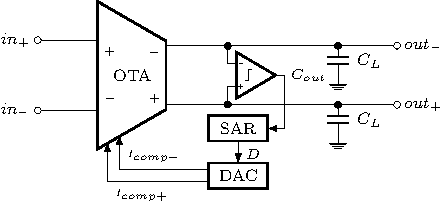
\includegraphics[scale=1]{fdota.pdf}\\
\end{center}
\caption 
{ \label{fig:fdota} 
Schemat blokowy FDOTA z cyfrową kalibracją napięcia niezrównoważenia.}
\end{figure}
\begin{figure}[!h]
  \begin{center}
  	\setlength{\tabcolsep}{0pt}
  	\begin{tabular}{ll}
  		(a) & (b)\\
  		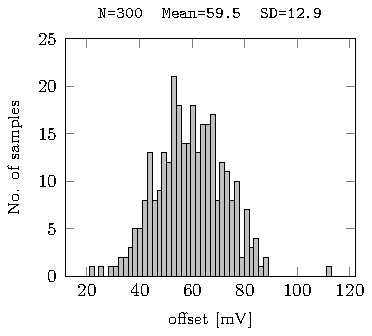
\includegraphics[height=5.2cm]{hist1.pdf}&
  		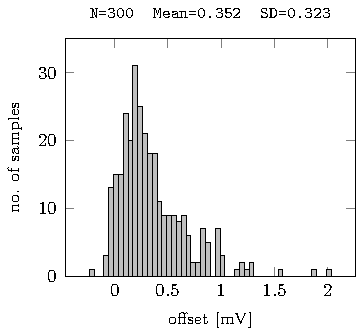
\includegraphics[height=5.2cm]{hist2.pdf}\\
  	\end{tabular}
  \end{center}
\caption
{ \label{fig:otah1} 
Rozrzut napięcia niezrównoważenia FDOTA: (a) bez kalibracji, (b) z 9-bitową kalibracją.}
\end{figure} 


\pagebreak


\section{Składanie wzorów}
\label{sec:wzory}
Jedną z wielu zalet {\LaTeX}-a, jak przystało na system składu publikacji naukowych, jest tryb matematyczny. W tym podrozdziale pokazano szereg przykładów użycia podstawowych konstrukcji tego trybu.

\subsection{Formuły w osobnych wierszach}
Podstawowym sposobem składania wzorów jest umieszczanie ich w osobnym wierszu. Wzory powinny być numerowane, tak jak to widać w poniższy przykładzie:
\begin{equation}
y= \frac{x-1}{x+2} 
\end{equation}
Automatyczną numerację uzyskujemy stosując otoczenie \texttt{\textbackslash begin\{equation\}\dots\textbackslash end\{equation\}}.
Umieszczenie etykiety umożliwi łatwe odwoływanie się do wzoru w~tekście, np. do formuły \ref{Eq:frac}.

\subsection{Formuły osadzone w tekście}
W najprostszym przypadku wzory mogą być integralną częścią akapitu, np. $E=mc^2$. Trzeba jednak pamiętać, że takie rozwiązanie stosujemy tylko do bardzo prostych (pomocniczych) zależności. Taka formuła jest trudna do odnalezienia, nie można uzyskać do niej odsyłacza a jeśli jest bardziej rozbudowana "rozpycha" tekst.

Szczególnie niekorzystnie  prezentują się osadzone w tekście ułamki ze względu na zmniejszony stopień pisma,  np. $y= \frac{x-1}{x+2}$. Jeśli zdecydujemy się temu zaradzić stosując polecenie \texttt{dfrac} zamiast \texttt{frac}, np.:  $y=\dfrac{x-1}{x+2}$, to znacząco zaburzona zostanie wielkość odstępów międzywierszowych, przez co tekst prezentuje się w sposób mało profesjonalny.

\subsection{Ułamki z ukośnikiem}
Proste ułamki lub miana można zapisać z wykorzystaniem ukośnika, np.: $\sfrac{1}{3}$, $\sfrac{1}{n}$, $\sfrac{V}{A}$.



\subsection{Indeksy górne i dolne}
Często spotykane są wyrażenia, w których stosowane są indeksy górne i dolne, np.:
\begin{equation}
a_{1},\ a_{i_{1}},\ a^{2},\ a^{b^{c}},\ a^{i_{1}},\
a_{i} + 1,\ a_{i + 1},\ a_{2}^{1},\ a^{2}_{1}
\end{equation}


\begin{equation}
x_{1} + x_{2} + \dots + x_{n}
\end{equation}


\subsection{Nawiasy i ograniczniki}
Szereg symboli takich jak nawiasy występuje w kilku odmianach różniących się wielkością. np.:
\[
( \dots \big( \dots \Big( \dots \bigg( \dots \Bigg(
\]
Zastosowanie "dużych" symboli poprawia czytelność złożonych formuł, np.: 
\[
F(x) |^{b}_{a} \dots
F(x) \bigr|^{b}_{a} \dots
F(x) \Bigr|^{b}_{a}
\]

\[
[ \sum_i a_i ]^{1/p} \dots  \left[ \sum_i a_i \right]^{1/p} \dots  \bigg[ \sum_i a_i \bigg]^{1/p} \dots  \Bigg[ \sum_i a_i \Bigg]^{1/p}
\]


\section{Ułamki piętrowe}

Zastosowanie zwykłego polecenia \texttt{frac} nie daje dobrych rezultatów:
\begin{equation}
  x = a_0 + \frac{1}{a_1
          + \frac{1}{a_2
          + \frac{1}{a_3 + \frac{1}{a_4} } } }
\end{equation}
W takiej sytuacji należy zastosować instrukcję \texttt{cfrac}:
\begin{equation}
  x = a_0 + \cfrac{1}{a_1
          + \cfrac{1}{a_2
          + \cfrac{1}{a_3 + \cfrac{1}{a_4} } } }
\end{equation}

\section{Justowanie wzorów}
Jeśli w tekście występuje kolejno kilka formuł to powinny one być wyjustowane względem siebie. Efekt ten uzyskuje się za pomocą otoczenia \texttt{\textbackslash begin\{align\}\dots\textbackslash end\{align\}}. W~formułach umieszczany jest symbol "\&", którego położenie wyznacza punkt odniesienia w każdej z~nich. Poniżej kilka przykładów wyjustowanych formuł.
\begin{align}
r^{2} &= s^{2} + t^{2}, \label{Eq:Pyth}\\
2u + 1 &= v + w^{\alpha}, \label{Eq:alpha}\\
x &= \frac{y + z}{\sqrt{s + 2u}};\label{Eq:frac}
\end{align}
\begin{align}
h(x) &= \int \left( \frac{f(x) + g(x)}{1+ f^{2}(x)} + \frac{1+ f(x)g(x)}{\sqrt{1 - \sin x}} \right) \, dx\label{E:longInt}=\\
&= \int \frac{1 + f(x)}{1 + g(x) } \, dx - 2 \tan^{-1}(x-2)\notag
\end{align}
W niektórych przypadkach samo justowanie nie wystarcza, np. podczas składania wzoru funkcji określonej przedziałami. W takim przypadku korzystamy z otoczenia \texttt{\textbackslash begin\{cases\}\dots \textbackslash end\{cases\}}. 
\begin{equation}
f(x)=
\begin{cases}
-x^{2}, &\text{if $x < 0$;}\\
\alpha + x, &\text{if $0 \leq x \leq 1$;}\\
x^{2}, &\text{otherwise.}
\end{cases}
\end{equation}



\section{Ingerowanie w skład dokumentu}
{\LaTeX} stara się rozmieścić tekst i inne elementy takie jak tabele, ilustracje czy wzory tak, aby uzyskać najlepszy efekt. Zdarza się jednak, np. kiedy blisko siebie występuje  duża liczba rysunków, że trzeba zaingerować  w układ pracy. 
\subsection{Kotwiczenie rysunków i tabel}
Jedną z najczęściej spotkanych sytuacji jest wymuszenie konkretnej pozycji ilustracji lub tabeli. W~tym celu należy definicję obiektu, czyli otoczenie \texttt{table} lub \texttt{figure}, uzupełnić o opcje wskazujące pożądaną lokalizację obiektu: \texttt{\textbackslash begin\{table\}\textbf{[!h]}},	\texttt{\textbackslash begin\{figure\}\textbf{[!h]}}. Litera \textit{h} jest skrótem od \textit{here}. Wykrzyknik nakazuje zaniechanie stosowania standardowych reguł rozmieszczania rysunków i tabel.

\subsection{Wymuszanie złamania strony}
Można wymusić złamanie strony w~konkretnym miejscu wstawiając polecenie  \texttt{\textbackslash pagebreak[\textit{n}]} (gdzie opcjonalny parametr \textit{n}=1\dots 4), które  {\LaTeX} interpretuje jako życzenie by zakończyć w tym miejscu stronę, tym silniejsze im większa jest wartość \textit{n}. 

\subsection{Wymuszanie złamania wiersza}
W celu wymuszenia przejścia do nowego wiersza \textit{bez rozpoczynania nowego akapitu} można zastosować polecenie \texttt{\textbackslash\textbackslash} lub \texttt{\textbackslash newline}.

\subsection{Zapobieganie wstawianiu wcięcia akapitowego}
Czasem (np. w sytuacji cytowania w podrozdziale \ref{fonty}) chcemy wstawić wiersz odstępu i jednocześnie uniknąć rozpoczęcia nowego akapitu. Wtedy na początku bloku tekstu wstawiamy polecenie \texttt{\textbackslash noindent}.

\subsection{Zapobieganiu przenoszeniu do nowego wiersza}
{\LaTeX} składając akapity stosuje automatyczne dzielenie i przenoszenie wyrazów, zgodnie z~regułami obowiązującymi w~języku, w jakim tworzony jest dokument. Zdarza się niekiedy, że zostaje rozdzielony   w ten sposób tekst, którego nie chcemy dzielić, np.: adres internetowy, stała fizyczna, itp. Można zapobiec dzieleniu słów i~przenoszeniu do nowego wiersza umieszczając tekst jako argument polecenia  \texttt{\textbackslash mbox\{\dots \}}. Poniżej przykład takiej sytuacji.
\vskip12pt
\textit{TeXstudio} jest dostępne nieodpłatnie na wszystkie platformy systemowe  na \url{http://texstudio.sourceforge.net/}.
\vskip12pt
\textit{TeXstudio} jest dostępne nieodpłatnie na wszystkie platformy systemowe  na \mbox{\url{http://texstudio.sourceforge.net/}}.

\subsection{Znaki specjalne}
Zdarza się że, musimy użyć słowa, które zawiera znak specjalny {\LaTeX}-a. Przykładem takiej sytuacji jest cytowanie nazwy pliku, która zawiera znak podkreślenia  "\_", np. w nazwie pliku \textit{praca\_dyplomowa.tex}. Wtedy należy taki znak poprzedzić odwróconym ukośnikiem czy znakiem \textbackslash.

\newpage
\section{Spis literatury}
Spis literatury generowany jest automatycznie, na podstawie umieszczonych w tekście odsyłaczy do rekordów bazy bibliograficznej.  
\subsection{Baza bibliograficzna w formacie \BibTeX}
Baza bibliograficzna w formacie \BibTeX jest w istocie plikiem tekstowym (o nazwie zwyczajowo zakończonej przez rozszerzenie \texttt{.bib}) zawierającym rekordy opisujące poszczególne pozycje. Praktycznie wszystkie wydawnictwa dostarczają referencji w formacie  \BibTeX, tak więc skompletowanie odpowiednio sformatowanej bazy bibliograficznej nie będzie nastręczało żadnych trudności. Każdy rekord w bazie musi zawierać  identyfikujący go unikalny klucz (etykietę). W podanym poniżej przykładzie są to \texttt{Pastre2006}, \texttt{Pastre2009}, \texttt{Pelgrom1989} i \texttt{wikibook}. 

{\footnotesize \begin{verbatim} 
@BOOK{Pastre2006,
  author = {Marc Pastre and Maher Kayal},
  title = {Methodology for the Digital Calibration of Analog Circuits and Systems: with 
  Case Studies (The Springer International Series in Engineering and Computer Science)},
  year = {2006},
  publisher = {Springer},
  isbn = {1402042523},
  url = {http://www.amazon.com/Methodology-Digital-Calibration-Circuits-Systems/dp/}
}
@INPROCEEDINGS{Pastre2009,
  author = {Pastre, M. and Kayal, M.},
  title = {Methodology for the digital calibration of analog circuits and systems 
  using sub-binary radix DACs},
  booktitle = {Mixed Design of Integrated Circuits Systems, 2009. MIXDES '09. MIXDES-16th
  International Conference},
  year = {2009},
  pages = {456-461},
  keywords = {analogue integrated circuits;calibrationy}
}
@ARTICLE{Pelgrom1989,
  author = {Pelgrom, M. J M and Duinmaijer, Aad C J and Welbers, A.P.G.},
  title = {Matching properties of MOS transistors},
  year = {1989},
  volume = {24},
  number = {5},
  pages = {1433-1439},
  issn = {0018-9200},
  journal = {Solid-State Circuits, IEEE Journal of},
  keywords = {MOS integrated circuits;insulated gate field effect transistors}
}
@WWW{wikibook,
  author = {Wikibooks},
  title = {LaTeX -- Wikibooks{,} The Free Textbook Project},
  year = {2012},
  url = {http://en.wikibooks.org/wiki/LaTeX}
}
\end{verbatim}
}

Bazę bibliograficzną można przygotować przy pomocy dowolnego edytora tekstowego lub specjalnego programu, np. \textit{JabRef} (\url{http://www.jabref.org/}).

\subsection{Odsyłacze}
W celu umieszczenia w tekście odsyłacza do konkretnej pozycji (lub grupy pozycji) należy użyć polecenia \texttt{\textbackslash cite\{klucz1,klucz2,\ldots \}}. Przykładowo,  umieszczenie w jednym miejscu odsyłaczy do dwóch pozycji wygląda następująco: \texttt{\textbackslash cite\{Pastre2006,Pelgrom1989\}}, co po przetworzeniu  da następujący efekt: \cite{Pastre2006,Pelgrom1989}. W przypadku sekwencji trzech odsyłaczy do kolejnych pozycji \texttt{\textbackslash cite\{Pastre2006,Pastre2009,Pelgrom1989\}}  efektem będzie \cite{Pastre2006,Pastre2009,Pelgrom1989}. W tym drugim przypadku wykryta została sekwencja odsyłaczy do  kolejnych pozycji literatury i automatycznie zastąpiono ją przedziałem indeksów. 

\subsection{Generowanie spisu literatury}
Wygenerowanie spisu literatury wymaga kilku przebiegów kompilatora (np. \texttt{pdflatex}, \texttt{lualatex}). Wynika to z faktu, że w trakcie przetwarzania  tekstu nie są jeszcze znane wszystkie odwołania do pozycji bibliografii. 

Po każdym przebiegu kompilatora tworzony jest pomocniczy plik (o rozszerzeniu \texttt{.aux}) zawierający klucze cytowanych pozycji. Dopiero na tej podstawie specjalny program \texttt{bibtex} może wygenerować zestawienie cytowanych pozycji bibliografii (plik z rozszerzeniem \texttt{.bbl}). To zestawienie jest wykorzystywane w kolejnym przebiegu kompilatora do wygenerowania rozdziału \textit{Bibliografia} w miejscu, w którym tekst zawiera polecenie \texttt{\textbackslash bibliography\{nazwa\_bazy\_bibliograficznej\}} oraz zastąpienia odsyłaczy identyfikatorami. Postać identyfikatorów zależy od przyjęto stylu formatowania bibliografii. W tym dokumencie zastosowany najprostszy styl czyli oznaczenie kolejnych pozycji spisu literatury kolejnymi liczbami (polecenie \texttt{\textbackslash bibliographystyle\{plainurl\}}).

Taka procedura całkowicie uwalnia użytkownika od konieczności samodzielnego wstawiania indeksów oraz bardzo kłopotliwego i podatnego na błędy korygowania tych indeksów po każdej modyfikacji bazy bibliograficznej.    

Znacznym ułatwieniem w tej sytuacji jest zastosowanie "inteligentnego" środowiska (np. \mbox{\textit{TeXStudio}}), które samodzielnie wywołuje w poprawnej kolejności wszystkie niezbędne programy w celu wygenerowania aktualnego zestawienia bibliografii. 

Jeśli zajdzie potrzeba wymuszenia ponownej generacji bibliografii należy usunąć plik \texttt{.bbl} oraz zaktualizować datę modyfikacji bazy bibliograficznej a następnie  uruchomić przetwarzanie dokumentu.




%%%%%%%%%%%%%%%%%%%%%%%%%%%%%%%%%%%%%%%%%%%%%%%%%%%%%%%%%%%%%%%%%%%%%%%%%%%%%%%%%%%%%%%%%
%%%%%%%%%%%%%%%%%%%%%%%%%%%%%%%%%%%%%%%%%%%%%%%%%%%%%%%%%%%%%%%%%%%%%%%%%%%%%%%%%%%%%%%%%


%%% Polecenie \nocite{*} spowoduje umieszczenie w bibliografii wszystkich pozycji z bazy 
%%% nie zależnie od tego czy w tekście umieszczono do nuch odsyłacze. 
%\nocite{*}
\bibliographystyle{../bibliografia/plainurl}
\bibliography{../bibliografia/spis}

%%%%%%%%%%%%%%%%%%%%%%%%%%%%%%%%%%%%%%%%%%%%%%%%%%%%%%%%%%%%%%%%%%%%%%%%%%%%%%%%%%%%%%%%%

\cleardoublepage
\printnoidxglossary[nopostdot, sort=def, title=Wykaz symboli i skrótów]
%%%%%%%%%%%%%%%%%%%%%%%%%%%%%%%%%%%%%%%%%%%%%%%%%%%%%%%%%%%%%%%%%%%%%%%%%%%%%%%%%%%%%%%%%


%%%%%%%%%%%%%%%%%%%%%%%%%%%%%%%%%%%%%%%%%%%%%%%%%%%%%%%%%%%%%%%%%%%%%%%%%%%%%%%%%%%%%%%%%
\cleardoublepage
\listoffigures
%%%%%%%%%%%%%%%%%%%%%%%%%%%%%%%%%%%%%%%%%%%%%%%%%%%%%%%%%%%%%%%%%%%%%%%%%%%%%%%%%%%%%%%%%


%%%%%%%%%%%%%%%%%%%%%%%%%%%%%%%%%%%%%%%%%%%%%%%%%%%%%%%%%%%%%%%%%%%%%%%%%%%%%%%%%%%%%%%%%
\cleardoublepage
\listoftables
%%%%%%%%%%%%%%%%%%%%%%%%%%%%%%%%%%%%%%%%%%%%%%%%%%%%%%%%%%%%%%%%%%%%%%%%%%%%%%%%%%%%%%%%%
%\cftinserthook{lot}{BREAK}
\cleardoublepage

\appendix
%\addappheadtotoc
\appendixpage
\appendixtableofcontents

% tutaj dodatki o ile istnieją
\chapter{Tekst źródłowy programu}


\begin{lstlisting}[language=VHDL,xleftmargin=0pt,  backgroundcolor={\color{white}}, caption={}, frame=""]
library ieee;
use ieee.std_logic_1164.all;
use ieee.std_logic_unsigned.all;
use ieee.std_logic_arith.all;

entity wave is
port (
  clk, reset : in std_logic;                           
  t_l, t_h   : in std_logic_vector(31 downto 0);  
  w          : out std_logic);
end wave;

architecture rtl of wave is
type FSM is (IDLE, PH, PL);
signal state, next_state: FSM;
signal timer : std_logic_vector(31 downto 0);
signal resetc: std_logic;

begin
RS_PROC:
process (clk, reset)
begin
  if (reset='0') then 
    state <= IDLE;
  elsif (rising_edge(clk)) then
    state <= next_state;
  end if;
end process;


NS_PROC:
process (state, t_l, t_h, timer)
begin
  case state is
  when  idle =>
  if (t_l = 0 or t_h = 0) then 
    next_state <= idle;
  else 
    next_state <= PH;
  end if;
  
  when PH =>  
  if (timer < t_h - 1) then  
    next_state <= PH;
  else
    next_state <= PL;
  end if;
    
  when PL =>
  if (timer < t_l - 1) then
    next_state <= PL;
  else
    next_state <= PH;    
   end if;    
end case;
end process;


DW_PROC:
process (state)
begin
  if    (state = PH) then   w <= '1';
  elsif (state = PL) then   w <= '0';
  end if;
end process;
end if;
end process;
end rtl;
\end{lstlisting}
\chapter{Model VHDL projektu}

\begin{lstlisting}[language=VHDL, xleftmargin=0pt, backgroundcolor={\color{white}}, caption={}, frame=""]
library ieee;
use ieee.std_logic_1164.all;
use ieee.std_logic_unsigned.all;
use ieee.std_logic_arith.all;

entity shift_reg is
generic(N: integer range 0 to 32 := 8);
port (
clk, reset, load  : in  std_logic;
pos, reg_in       : in  std_logic_vector(N-1 downto 0);
reg_out           : out std_logic_vector(N-1 downto 0));
end shift_reg;

architecture rtl of shift_reg is
signal rejestr: std_logic_vector(N-1 downto 0);

begin
process (clk, reset, load, reg_in)
begin
  if (reset = '0') then 
    rejestr <= (others => '0');
   elsif (load = '0') then
     rejestr <= reg_in;
   elsif (rising_edge(clk)) then
     rejestr (N-1 downto conv_integer(pos)) <= rejestr(N-1-conv_integer(pos) downto 0);
     rejestr (conv_integer(pos) downto 0)   <= (others => '0');
  end if;
end process;

reg_out <= rejestr;
end rtl;
\end{lstlisting}



\end{document}

